%%%%%%%%%%%%%%%%%%%%%%%%%%%%%%%%%%%%%%%%%%%%%%%%%%%%%%%%
%%%  Manuscript 8 - Dendronotus CPG Model
%%%  Based on Cell Press LaTeX template v1.10
%%%
%%%  Version 8: Revised framing to acknowledge Getting's
%%%  precedent on network oscillators and slow synaptic
%%%  mechanisms. Reoriented claims to emphasize genuine
%%%  novelty (controllability, network hysteresis terminology,
%%%  presynaptic vs postsynaptic modulation prediction).
%%%%%%%%%%%%%%%%%%%%%%%%%%%%%%%%%%%%%%%%%%%%%%%%%%%%%%%%

\documentclass[12pt,letterpaper]{article}
\usepackage[a4paper, total={7in, 10in}]{geometry}
\renewcommand{\familydefault}{\sfdefault}
\usepackage{graphicx}
\usepackage{helvet}
\usepackage{authblk}
\usepackage{hyperref}
\usepackage{amsmath}
\usepackage{amssymb}
\usepackage{orcidlink}
\usepackage[super,comma,sort&compress]{natbib}
\bibliographystyle{numbered}
\usepackage[right]{lineno} \linenumbers

\makeatletter
\renewcommand{\maketitle}{\bgroup\setlength{\parindent}{0pt}
\begin{flushleft}
  \textbf{\@title}

  \@author
\end{flushleft}\egroup}
\makeatother

%%% Title
\title{Network oscillations explain flexible burst frequency control in the Dendronotus Iris swim central pattern generator}
\title{Slow synaptic dynamics promote resilience and regulate burst frequency in the Dendronotus iris swim central pattern generator [model]}
\date{}

%%% Authors and Affiliations
\author[1,2,5,*]{James Scully}
\author[3]{Akira Sakurai}
\author[4]{Paul S. Katz}
\author[1,2]{Andrey L. Shilnikov}

\affil[1]{Neuroscience Institute, Georgia State University, 100 Piedmont Ave., Atlanta, GA 30303, USA}
\affil[2]{Department of Mathematics \& Statistics, Georgia State University, 25 Park Pl., Atlanta, GA 30303, USA}
\affil[3]{Department of Biology, Georgia State University, Atlanta, GA 30303, USA}
\affil[4]{Department of Biology, University of Massachusetts Amherst, Amherst, MA, USA}
\affil[5]{Lead contact}

\affil[*]{Correspondence: jamesjscully@gmail.com}

\begin{document}

\maketitle

%%% Summary
\section*{SUMMARY}

Rhythmic behaviors, like swimming, rely on Central Pattern Generators (CPGs) that must be both robust and resilient to perturbation and tunable by descending commands.
Early work established that some CPGs act as ``network oscillators'' -- {\bf collectively generating emergent rhythm} through synaptic interactions rather than due to {\bf dedicated} cellular pacemakers alone \cite{Getting1983delayed, Getting1989}.
While pacemaker-driven and {\bf [bistable] half-center oscillators??} have been extensively studied, the mechanisms enabling \textit{smooth and broad frequency control} in network oscillators remain less well characterized.

We address this question through computational modeling of the swim CPG of the nudibranch \textit{Dendronotus iris}, a four-cell circuit controlled by Si1 command neurons.
We identify contralateral excitatory-inhibitory (E/I) modules as the core {\em rhythmogenic} engine {\bf symmetrically built-in the swim CPG}.

These modules operate in an ``almost-oscillatory'' {\bf [love it or on the oscillatory edge]} regime where rhythm emerges through network-level hysteresis: slow synaptic accumulation creates the history-dependence in post-synaptic neurons giving rise to  bistability and oscillations in E/I modules and the whole CPG. 

Progressive network assembly reveals that E/I modules, combined/enhanced with two half-center-oscillators between left/right constituent interneurons [Si2s and Si3s] bonded by reciprocal inhibition, constitute the circuit capable for emergent and resilient rhythm generation.

Its theoretical/mathematical model reproduces experimental perturbation responses without parameter fitting, confirming its distributed robustness or behavioral stability.
We further demonstrate that presynaptic modulation of transmitter release rate enables smooth 
network frequency control, whereas postsynaptic conductance modulation yields threshold-like transitions.
These findings provide a mechanistic account of how network oscillators achieve the {\bf graded}frequency control long observed in motor systems.


%%% Keywords
\section*{KEYWORDS}

central pattern generator, Dendronotus iris, neural oscillation, synaptic dynamics, frequency modulation, half-center oscillator, computational model, neuron-modulation, resilience, network oscillations, network hysteresis, behavioral stability, adaptability, emergent oscillations   

%%% Introduction
\section*{INTRODUCTION}

Animals swim, walk, and breathe in steady rhythms.
These rhythmic behaviors rely on central pattern generators (CPGs), neural circuits that can generate coordinated motor output in the absence of patterned sensory input.
Classic fictive preparations established that the temporal structure of motor patterns can arise centrally, motivating the study of CPGs as autonomous yet context-sensitive networks \cite{Wilson1961, MarderCalabrese1996, Kiehn2006}.
Early work on invertebrate CPGs recognized two broad architectures: pacemaker-driven oscillators, where intrinsically bursting neurons provide rhythmic drive, and network oscillators, where rhythm emerges from synaptic interactions among non-bursting neurons \cite{Getting1989}.
The Tritonia swim CPG exemplified the latter---none of its neurons exhibited intrinsic bursting, yet the network generated robust rhythm through ``delayed excitation'' and other slow synaptic mechanisms \cite{Getting1983delayed, Getting1983network}.
As research characterized diverse ionic currents underlying cellular bursting \cite{Rinzel87b, RL87}, attention shifted toward pacemaker-driven systems and the modulation of intrinsic properties.
The question of how network oscillators achieve \textit{smooth, graded frequency control} has received less systematic attention.

The swim CPG of the nudibranch \textit{Dendronotus iris} presents a compact instance of this problem: four neurons, none capable of intrinsic bursting, generate robust left--right alternation whose frequency varies smoothly under a single command signal.
Like its Tritonia relatives, the \textit{Dendronotus} circuit relies on synaptic rather than cellular mechanisms for rhythm generation.
We propose that such circuits exploit what we term \textit{network hysteresis}: slow synaptic dynamics assume the role of the slow intrinsic variable found in cellular bursters, accumulating across network partners to create history-dependent transitions between collective activity states.
This terminology builds on Getting's (1983) characterization of ``delayed excitation,'' providing a unifying concept that connects slow synaptic accumulation to the hysteresis framework used to analyze cellular bistability.

Intrinsically bursting neurons generate rhythm through cellular hysteresis: active and silent states coexist across a range of a slow intrinsic variable such as intracellular calcium, and the variable's drift between these states drives phase transitions within a single cell \cite{Rinzel87b, RL87}.
This mechanism imposes rhythm but couples frequency tightly to burst shape.
Half-center oscillators enforce alternation through reciprocal inhibition \cite{brown}, with escape, release, or post-inhibitory rebound governing phase transitions \cite{Wang-Rinzel-92, SKM94}.
Skinner, Kopell, and Marder (1994) showed that when phase transitions depend on intrinsic cellular mechanisms, network frequency is insensitive to synaptic parameters; when transitions depend on synaptic mechanisms, frequency becomes tunable through synaptic properties.
This distinction suggests that network oscillators lacking cellular pacemakers may be inherently more amenable to frequency control---a possibility we explore quantitatively.

Network oscillators can be understood as assemblies of canonical subnetwork building blocks \cite{Getting1989}.
Excitatory-inhibitory (E/I) coupling represents one such building block capable of generating oscillations through network interaction alone \cite{WilsonCowan1972}.
Wilson and Cowan (1972) showed that E/I networks can exhibit oscillations and hysteresis, but their models operate on cortical timescales with fast synapses tuned for gamma rhythms.
We propose that network hysteresis, arising from slow synaptic dynamics within E/I subnetworks, provides the mechanism by which network oscillators achieve robust, graded frequency control at CPG timescales.

CPG circuits exhibit degeneracy: similar output despite varied synaptic and cellular properties \cite{MarderCalabrese1996, Marder2011}.
Neuromodulators reconfigure circuits without changing wiring \cite{NusbaumBeenhakker2002, JingWeiss2005}, but adaptability also demands that frequency be tunable.

Slow synaptic dynamics provide a plausible substrate for such control.
Repeated presynaptic firing can facilitate or depress transmission over tens to hundreds of milliseconds, timescales comparable to burst durations \cite{zucker2002short, jackman2017mechanisms}.
These dynamics reshape effective coupling without requiring large changes in baseline synaptic conductance.
Neuromodulators frequently target presynaptic release machinery, thereby tuning the timing and gain of transmission in ways that can strongly reshape circuit dynamics \cite{NadimBucher2014}.
In \textit{Tritonia diomedea}, serotonergic interneurons within the swim CPG show this principle directly: spike timing--dependent facilitation of their own synapses grants the network graded frequency control without an external modulatory system \cite{katz1994dynamic, sakurai2003spike}.

In \textit{Dendronotus iris}, experiments have characterized the swim CPG's connectivity, command neurons, and responses to targeted perturbations \cite{SakuraiKatz2016, sakurai2019command}.
The command-like Si1 neurons both initiate swimming and modulate swim frequency, providing the unified control signal that the circuit architecture must accommodate.

Here we build a computational model of the \textit{Dendronotus} swim CPG constrained by its known circuit topology, cellular properties, and synaptic kinetics.
Our analysis reveals three principal findings.
First, rhythm generation depends on contralateral E/I modules operating near an oscillatory threshold: ``almost-oscillatory'' subcircuits whose slow synaptic feedback creates the temporal framework for bursting.
Second, this distributed architecture confers resilience: the model reproduces experimental perturbation responses without parameter adjustment, confirming that no single neuron is essential for rhythm maintenance.
Third, neuromodulatory control of presynaptic release kinetics enables smooth frequency tuning, whereas postsynaptic conductance modulation produces abrupt, threshold-like transitions.
These results establish that network hysteresis, emergent from slow synaptic dynamics rather than cellular bistability, provides a robust yet flexible substrate for CPG function---reconnecting with insights from the early characterization of network oscillators while providing new mechanistic detail on how such circuits achieve controllability.


%%% Results
\section*{RESULTS}

\subsection{Circuit architecture: E/I modules as the oscillatory core}

How does a network of non-bursting neurons generate robust rhythmic output?
The \textit{Dendronotus} swim CPG achieves this through network hysteresis: slow synaptic feedback within contralateral E/I modules creates the history-dependence that individual neurons lack, driving alternation between left and right activity states (Fig.~\ref{fig:ei_mechanism}).
We constructed a computational model of this four-cell network by integrating validated two-cell subnetworks---half-center oscillators (HCOs) and E/I modules---following the approach developed in \cite{scully2024pairing}.

The circuit architecture distributes rhythmogenic function across the network rather than concentrating it in pacemaker cells (Fig.~\ref{fig:ei_mechanism}A).
Each E/I module pairs an excitatory Si3 neuron with a contralateral Si2 neuron in a ``twisted'' configuration that crosses the midline: Si3R drives Si2L and Si3L drives Si2R.
Within each module, Si3 provides excitatory drive through a logistic synapse with relatively fast kinetics, while Si2 returns slower inhibitory feedback through a logistic synapse.
This delayed negative feedback loop constitutes the conceptual and computational primitive of the swim network---the fundamental building block from which network-level bursting emerges.

Critically, each E/I module is tuned to be ``almost-oscillatory'': when isolated, it exhibits damped oscillations or subthreshold rhythmic fluctuations rather than sustained limit cycles.
This design means that no single component can generate rhythm autonomously; network coupling is required to recruit the modules into coordinated bursting.
The two HCOs (Si3L$\leftrightarrow$Si3R and Si2L$\leftrightarrow$Si2R) provide reciprocal inhibition that enforces anti-phase alternation between left and right sides.
Unlike classical HCO-based CPGs where reciprocal inhibition drives rhythm generation, these connections function primarily as stabilizers---the E/I modules supply the oscillatory drive.
Weak electrical coupling between E/I partners (Si3R$\leftrightarrow$Si2L and Si3L$\leftrightarrow$Si2R) provides rapid voltage coordination within each module and contributes to network resilience.

The kinetic asymmetry between fast excitation and slow inhibition is visible in the neurotransmitter traces (Fig.~\ref{fig:ei_mechanism}B): excitatory synaptic variables (red) rise and fall rapidly with each spike, while inhibitory variables (blue) accumulate gradually across the burst and decay slowly during interburst intervals.
This temporal separation means that Si3 excitation recruits Si2 activity quickly, but the inhibition that eventually terminates Si3 firing builds over hundreds of milliseconds---the timescale that sets burst duration.

These synaptic timescales are not arbitrary modeling choices but reflect dynamics observed in the biological circuit.
Figure~\ref{fig:synaptic_timescales} demonstrates correspondence between model and experimental recordings: current injection into Si2R evokes dual-timescale responses in its network partners.
The fast $\alpha$-synapse produces IPSPs in Si2L that rise and decay within tens of milliseconds.
Electrical coupling appears as an immediate voltage deflection in Si3L that precedes the slower chemical response.
The logistic synapse from Si2 to Si3 accumulates over repeated stimulation, producing delayed inhibition that builds across hundreds of milliseconds.
Together, fast reciprocal inhibition, slow E/I feedback, and near-instantaneous electrical coupling establish the temporal framework within which network bursting emerges.

\subsection{Network assembly and rhythm emergence}

Having established the circuit architecture, we now demonstrate how progressive integration of synaptic connections generates the complete swim CPG.
The four-cell network was constructed by sequentially activating synapses, revealing which interactions are necessary and sufficient for rhythm generation (Fig.~\ref{fig:assembly}).

In the initial configuration (Fig.~\ref{fig:assembly}A), the four interneurons are uncoupled.
Si3 neurons fire tonically at approximately 50~Hz with elevated excitability modeling excitatory drive from Si1 command neurons, while Si2 neurons remain quiescent.
When fast excitatory synapses from Si3 to contralateral Si2 are activated (Fig.~\ref{fig:assembly}B), Si2 neurons transition to tonic firing.
Addition of slow inhibitory feedback from Si2 to Si3 (Fig.~\ref{fig:assembly}C) produces spike-frequency modulation within the contralateral E/I loops (Si3R$\leftrightarrow$Si2L and Si3L$\leftrightarrow$Si2R), but consistent with experimental observations \cite{SakuraiKatz2016}, these loops alone do not generate autonomous bursting.

Reciprocal inhibition between contralateral Si3 neurons (Fig.~\ref{fig:assembly}D) immediately produces burst alternation, organizing Si3 activity into 2--3 second bursts separated by hyperpolarized interburst intervals.
Si2 neurons exhibit corresponding burst episodes driven by their Si3 partners.
This demonstrates that the Si3 half-center oscillator, when combined with the E/I modules, provides the phase-switching mechanism that converts continuous E/I dynamics into discrete alternating bursts.

The complete network (Fig.~\ref{fig:assembly}E), incorporating reciprocal Si2 inhibition and weak electrical coupling between E/I pairs, generates stable antiphase alternation with 3--4 second bursts that match experimental recordings.
Importantly, the stable rhythm is robust to the order in which synaptic connections are activated, confirming that network topology rather than assembly history determines the final dynamics.
This distributed architecture---where no single component is solely responsible for rhythm generation---predicts that the network should tolerate transient disruptions.
We test this prediction against experimental recordings.

\subsection{Model validation and robustness testing through targeted perturbations}

To validate our computational model and assess network robustness, we reproduced key perturbation experiments from the original \textit{Dendronotus iris} swim CPG studies \cite{SakuraiKatz2016, sakurai2022bursting}.
Brief hyperpolarizing or depolarizing current pulses delivered to targeted interneurons during ongoing swim episodes test how the circuit responds to transient disruptions and whether it recovers its characteristic oscillatory pattern.
A robust network should maintain coordinated output despite perturbations and return rapidly to stable operation upon their removal.
Faithful reproduction of these experimental responses confirms that the model captures both the functional dynamics and the stability properties of the biological CPG.

Figure~\ref{fig:perturbation_responses} presents six perturbation experiments (panels A--F) that reveal distinct aspects of circuit resilience.
Across all conditions, the circuit recovers coordinated bursting once perturbations are removed, demonstrating that the network operates as a robust attractor.

Panel A shows that depolarizing Si3L produces immediate cessation of network bursting followed by rapid recovery.
The contralateral Si3R neuron becomes hyperpolarized due to strong reciprocal inhibition, and Si2R is silenced via the E/I inhibitory projection.
Panel B represents a special case: it is the only perturbation in which network bursting is not completely halted.
The targeted Si2R neuron is strongly inhibited, yet activity persists through alternative pathways---underscoring that the E/I modules, not individual neurons, constitute the core oscillatory engine.

Panel C shows both Si2 interneurons simultaneously hyperpolarized.
The circuit recovers, but restoration takes noticeably longer than in unilateral cases, highlighting the supporting role Si2 neurons play in stabilizing the rhythm.
Panel D applies a depolarizing pulse to Si3R, disrupting alternation; upon pulse termination, the circuit rapidly returns to its characteristic antiphase rhythm.

Panel E shows hyperpolarization of Si3R, which silences its electrical partner Si2L through gap junction coupling.
Panel F shows bilateral hyperpolarization of both Si3 neurons, which completely abolishes network activity.
Silencing both Si3 neurons eliminates excitatory drive to the Si2 neurons, which are configured near the threshold between tonic spiking and quiescence.
Upon removal of the hyperpolarizing pulses, the CPG rapidly restores the control rhythm, demonstrating that Si3 neurons are necessary to initiate network-level bursting.
Additional symmetric bilateral perturbation experiments further validate the model's dynamics (Supplementary Materials).

These perturbation experiments assumed elevated Si3 excitability to sustain ongoing bursting.
In the biological circuit, this drive originates from Si1 command neurons, whose control over network state we examine next.

\subsection{Top-down control and neuromodulation}

In the biological circuit, Si3 neurons are not intrinsically oscillatory but receive tonic excitatory drive from Si1 command neurons that initiate and sustain swim episodes \cite{sakurai2019command}.
We now examine a five-cell network configuration that incorporates Si1 control, with Si3 neurons set to quiescent baseline states that require Si1 excitation to become active.

\subsubsection{Si1 gating of network activity}

In \textit{Dendronotus iris}, Si1 neurons function as command-like neurons that initiate and terminate swim episodes \cite{sakurai2019command}.
They provide tonic excitatory drive to both Si3 neurons, which in turn activate the four-cell CPG through the contralateral E/I modules.
This hierarchical organization allows Si1 neurons to gate network state transitions while intrinsic CPG dynamics shape burst structure and left-right alternation.

Figure~\ref{fig:si1_neuromod}A summarizes the network architecture used for this analysis.
Si1 provides excitatory drive to both Si3 neurons and also modulates the Si3$\to$Si2 excitatory pathway, thereby coupling episode recruitment to burst-frequency regulation within the same command system.

\subsubsection{Neuromodulatory burst frequency control}

Beyond gating network activity, Si1 neurons regulate burst frequency in an activity-dependent manner.
Experimental recordings demonstrate that swim frequency increases with Si1 firing rate, establishing that the command signal encodes not merely on/off state but graded frequency information \cite{sakurai2019command}.
This observation motivates our exploration of how neuromodulation of synaptic properties in the Si3$\to$Si2 excitatory pathway could implement such graded control.
We compared two distinct mechanisms: presynaptic modulation of the logistic Si3$\to$Si2 accumulation-rate parameter $\alpha$, and postsynaptic modulation of the maximal effective conductance in the same pathway.

Figure~\ref{fig:si1_neuromod}B compares the biological Si1-rate versus burst-rate relationship with matched measurements extracted from representative model traces.
Both model variants capture the positive relationship between command-neuron firing and burst frequency, but the presynaptic model occupies the biological range more naturally across successive burst intervals, whereas the postsynaptic model is compressed toward higher burst frequencies for a broad range of Si1 firing rates.

Figure~\ref{fig:si1_neuromod}C shows the full gain scan during ongoing drive.
Presynaptic modulation produces a broader and smoother increase in burst frequency as gain increases.
Postsynaptic modulation also increases burst frequency, but the response is flatter over substantial parts of the scan and reaches a comparatively narrow high-frequency band.
Thus, both mechanisms can tune the active rhythm, but presynaptic modulation provides a more graded control landscape.

Figure~\ref{fig:si1_neuromod}E shows representative biological and model traces.
The biological recording establishes the empirical relationship between elevated Si1 firing and Si2 bursting, while the two model traces illustrate how the same Si1 drive can be translated into different burst statistics depending on whether modulation acts on release kinetics or effective conductance.

Taken together, these results support a restrained conclusion: Si1-mediated modulation of the Si3$\to$Si2 pathway is sufficient to regulate burst frequency during active swimming, and modulation of synaptic kinetics provides the closer match to the observed graded Si1-to-burst relationship.
This generates a testable prediction that pharmacological manipulations targeting presynaptic release machinery should produce smoother frequency tuning than manipulations acting primarily on postsynaptic conductance.


%%% Discussion
\section*{DISCUSSION}

Our findings demonstrate that slow synaptic dynamics play a central role in generating robust, adaptable rhythms in the \textit{Dendronotus iris} swim CPG.
Previous work established that synaptic properties shape CPG output \cite{Manor1997, NadimBucher2014}, but these studies examined circuits containing intrinsically bursting neurons or focused on synaptic amplitude rather than temporal dynamics.
The present work addresses a distinct question: in circuits lacking intrinsic pacemakers, how do slow synaptic kinetics regulate rhythmic output and enable smooth frequency control?

\subsection*{Reconnecting with early insights on network oscillators}

Our findings reconnect with foundational insights from early CPG research.
Getting (1983, 1989) demonstrated that the Tritonia swim CPG generates rhythm through ``delayed excitation''---slow synaptic mechanisms operating in a network where no neuron exhibits intrinsic bursting \cite{Getting1983delayed, Getting1983network, Getting1989}.
This work established the concept of the ``network oscillator'' and emphasized that rhythm generation could emerge from synaptic interactions alone.
As research subsequently characterized the rich repertoire of ionic currents underlying pacemaker-driven rhythms in systems like the stomatogastric ganglion, the importance of synaptic \textit{kinetics}---as distinct from synaptic strength---for frequency control received less systematic attention.

Our quantitative analysis of the Dendronotus circuit suggests that slow synaptic dynamics deserve renewed emphasis as primary regulators of network oscillator behavior.
We introduce the term ``network hysteresis'' to connect Getting's ``delayed excitation'' to the hysteresis framework commonly applied to cellular bistability: just as slow intrinsic variables create history-dependence in bursting neurons, slow synaptic accumulation creates history-dependence at the network level.
This terminology provides a unifying concept linking synaptic and cellular mechanisms within a common dynamical framework.

\subsection*{Presynaptic modulation provides smooth frequency control}

Presynaptic modulation of the accumulation rate parameter $\alpha$ in the logistic Si3$\to$Si2 excitatory synapses produces smooth, graded control of burst frequency (Fig.~\ref{fig:si1_neuromod}D), whereas postsynaptic modulation of $g_{syn}$ in the same synapses yields threshold-like transitions between oscillatory regimes (Fig.~\ref{fig:si1_neuromod}E).
From a control-theoretic perspective, presynaptic modulation creates a more favorable landscape: small changes in neuromodulatory input produce proportional changes in network output.

This distinction builds on Skinner, Kopell, and Marder's (1994) analysis showing that oscillation mechanisms relying on intrinsic cellular properties render frequency insensitive to synaptic parameters, while mechanisms relying on synaptic dynamics render frequency sensitive to those parameters \cite{SKM94}.
Our results extend this principle: in network oscillators lacking cellular pacemakers, frequency control naturally operates through synaptic mechanisms, and the \textit{kinetics} of transmission---not merely its strength---determine whether control is smooth or threshold-like.

Biologically, presynaptic modulation can be achieved through regulation of vesicle priming, calcium sensitivity, and release probability \cite{NeherBrose2018, jackman2017mechanisms}.
Activity-dependent modulation of release kinetics is well established in the related nudibranch \textit{Tritonia diomedea}, where serotonergic swim interneurons facilitate synaptic transmission through spike timing-dependent mechanisms \cite{katz1994dynamic, sakurai2003spike}.
That independent computational modeling of \textit{Dendronotus} predicts a similar reliance on facilitation suggests this may represent a conserved mechanism for rhythm control across gastropod swim CPGs.
\textit{Dendronotus} and \textit{Tritonia} diverged approximately 140 million years ago and evolved swimming independently, yet both appear to exploit slow synaptic dynamics for frequency regulation \cite{newcomb2012homologues}.
Comparative studies across nudibranch species with different body sizes, swim frequencies, and ecological niches could reveal whether facilitation parameters scale systematically with morphology or behavior.
Such scaling would support the hypothesis that synaptic timescales represent a primary target for evolutionary tuning of motor output.

Our model generates testable predictions: pharmacological agents that enhance or reduce release probability should produce smooth, graded changes in swim frequency, whereas agents targeting postsynaptic conductance should produce more abrupt transitions.

\subsection*{Network hysteresis and the functional properties of network oscillators}

The \textit{Dendronotus} swim CPG is assembled from ``almost-oscillatory'' subcircuits that individually exhibit subthreshold dynamics but collectively generate rhythmic output.
This architecture contrasts with CPG models based on intrinsically bursting pacemaker neurons \cite{plant81, Rinzel87b, RL87}, but aligns with Getting's characterization of the Tritonia network oscillator \cite{Getting1989}.
In our model, bursting emerges from network-level hysteresis created by slow synaptic accumulation and delayed feedback through the contralateral E/I modules.
Progressive assembly confirms this distributed design: the E/I modules combined with Si3 reciprocal inhibition constitute the minimal circuit for rhythm generation, while Si2 reciprocal inhibition and electrical coupling provide additional structure.

The perturbation experiments (Fig.~\ref{fig:perturbation_responses}) reveal that the resulting limit cycle is locally stable: following transient perturbations, the network returns to coordinated antiphase bursting.
This recovery occurs across diverse perturbation types---unilateral depolarization, unilateral hyperpolarization, and bilateral manipulations---indicating that the attractor basin is broad.
The one exception is bilateral Si3 hyperpolarization, which abolishes rhythmic activity entirely; this confirms that Si3 excitatory drive is necessary to maintain the network in the oscillatory regime.

The distributed architecture also confers what Marder and colleagues have termed degeneracy: the capacity to produce similar functional output from varied underlying parameters \cite{MarderGoaillard2006, Prinz2004}.
Our model reproduces experimental perturbation responses without parameter fitting, suggesting that the biological circuit may likewise tolerate parameter variation provided the essential synaptic interactions are preserved.
More directly, when Si2R is hyperpolarized (Fig.~\ref{fig:perturbation_responses}B), rhythmic activity persists through alternative pathways---the only perturbation condition in which bursting is not completely halted.
This observation supports the interpretation that multiple synaptic routes can sustain rhythm, a hallmark of degenerate circuit architecture.

A distinct property is adaptability: the capacity to adjust output frequency in response to modulatory signals.
Skinner, Kopell, and Marder (1994) showed that when phase transitions depend on intrinsic cellular mechanisms (escape or release from cellular bistability), network frequency is relatively insensitive to synaptic parameters; when transitions depend on synaptic mechanisms, frequency becomes tunable through those parameters \cite{SKM94}.
Because network hysteresis locates the slow variable in synaptic dynamics rather than cellular currents, frequency control naturally operates through synaptic modulation.
Our results confirm this: presynaptic modulation of release kinetics produces smooth, graded frequency changes (Fig.~\ref{fig:si1_neuromod}D), whereas postsynaptic conductance modulation produces threshold-like transitions (Fig.~\ref{fig:si1_neuromod}E).
The absence of cellular bistability thus enables controllability---frequency can be tuned through a single synaptic parameter without requiring coordinated changes across multiple intrinsic conductances.

These observations suggest a relationship between network hysteresis and functional circuit properties.
Emergent oscillations arise because slow synaptic accumulation creates the history-dependence required for state transitions in circuits lacking cellular pacemakers.
Local stability of the limit cycle ensures that transient perturbations do not permanently disrupt rhythm.
Degeneracy arises because rhythm generation depends on collective synaptic interactions that can be achieved through multiple parameter combinations.
Adaptability arises because the synaptic locus of the slow dynamics places frequency control within reach of neuromodulatory systems that target presynaptic release machinery \cite{NadimBucher2014}.

The ``almost-oscillatory'' design principle may also facilitate developmental adaptation.
As animals grow, swim frequency must decrease to match the longer body wavelengths required for efficient locomotion.
If rhythm generation depended on tightly coordinated cellular properties, developmental scaling would require simultaneous adjustment of multiple intrinsic conductances---a complex regulatory challenge.
By contrast, synaptic timescales can be tuned through changes in receptor subunit composition, vesicle pool dynamics, or presynaptic calcium handling, potentially providing a simpler developmental control point.
Tracking synaptic kinetics alongside body size during \textit{Dendronotus} development could test whether ontogenetic changes in facilitation timescales match the functional demands of body scaling.

\subsection*{Broader implications}

Rhythmic motor patterns must be continuously adjusted to meet changing demands while maintaining coordination.
Slow synaptic kinetics provide an ideal substrate for such regulation: their extended timescales create a temporal buffer that smooths the translation of modulatory signals into network output, preventing abrupt transitions that could destabilize coordinated movement.

This principle likely extends beyond invertebrate circuits.
Mammalian locomotor CPGs must vary walking speed smoothly from slow ambling to rapid running while maintaining interlimb coordination, and gait transitions must occur without loss of phase relationships \cite{Kiehn2006}.
Respiratory CPGs adjust breathing frequency across rest, exercise, and emotional states while preserving precise timing among respiratory muscles \cite{DelNegro2018}.
In each case, the circuit must balance stability against flexibility---precisely the trade-off that slow synaptic dynamics appear well-suited to mediate.
The neuromodulatory targeting of presynaptic release machinery, rather than postsynaptic conductances, may represent a general strategy for achieving smooth, reversible frequency control across these systems \cite{NadimBucher2014}.

Our findings suggest that understanding the temporal structure of synaptic transmission, not merely its strength, may be essential for deciphering how neuromodulators sculpt behavior.

\subsection*{Limitations}

Several limitations should be acknowledged.
Our validation emphasizes qualitative reproduction of experimental perturbation responses rather than statistical fitting of burst parameters.
Direct experimental evidence for whether Si1-driven frequency control operates through presynaptic or postsynaptic modulation remains to be established.
We model Si1 as a single neuron, whereas the biological system employs electrically coupled bilateral Si1L and Si1R neurons, and we omit sensory feedback and descending inputs beyond Si1.
The model's rapid recovery across diverse perturbation conditions (Fig.~\ref{fig:perturbation_responses}) provides functional evidence that the distributed architecture confers stability.


%%% Resource Availability
\section*{RESOURCE AVAILABILITY}

\subsection*{Lead contact}

Requests for further information and resources should be directed to and will be fulfilled by the lead contact, James Scully (jamesjscully@gmail.com).

\subsection*{Materials availability}

This study did not generate new materials.

\subsection*{Data and code availability}

\begin{itemize}
    \item This paper analyzes existing, publicly available data. The original experimental data are available from the cited sources.
    \item All original code has been deposited at GitHub (https://github.com/jamesjscully/Dendronotus) and is publicly available as of the date of publication.
    \item Any additional information required to reanalyze the data reported in this paper is available from the lead contact upon request.
\end{itemize}


%%% Acknowledgments
\section*{ACKNOWLEDGMENTS}

We thank the Brains \& Behavior Initiative at Georgia State University for support through a Brains \& Behavior pilot grant and for a Brains \& Behavior graduate fellowship awarded to J.~Scully.
We are grateful to the current and former members of the Shilnikov NeurDS (Neuro-Dynamical Systems) laboratory, including J.~Bosonetto, D.~Bloom, C.~Hinsley, Y.~Keleta, and Drs.~H.~Ju, D.~Alacam, and K.~Pusuluri for many helpful and inspiring discussions.
This work was supported by the National Science Foundation (NSF) under award IOS--1455527.

%%% Author Contributions
\section*{AUTHOR CONTRIBUTIONS}

Conceptualization, J.S. and A.L.S.;
Methodology, J.S. and A.L.S.;
Software, J.S.;
Investigation, J.S.;
Writing -- Original Draft, J.S.;
Writing -- Review \& Editing, J.S., A.S., P.S.K., and A.L.S.;
Visualization, J.S.;
Supervision, A.L.S.;
Funding Acquisition, A.L.S. and P.S.K.

%%% Declaration of Interests
\section*{DECLARATION OF INTERESTS}

The authors declare no competing interests.

%%% Declaration of Generative AI
\section*{DECLARATION OF GENERATIVE AI AND AI-ASSISTED TECHNOLOGIES}

During the preparation of this work, the authors used AI as a writing assistant and expedient editing of code for figures.
All ideas and concepts are our own.
The authors reviewed and edited all AI-generated content and take full responsibility for the content of the publication.

%%% Supplemental Information Index
\section*{SUPPLEMENTAL INFORMATION INDEX}

\begin{description}
  \item Figures S1--S2 and their legends in a PDF
  \item Table S1. Model parameters
\end{description}

\newpage

%%% Main Figure Titles and Legends
\section*{MAIN FIGURE TITLES AND LEGENDS}

%%% Figure 1: E/I Module Mechanism (fig1.jpg)
\begin{figure}[htbp]
\centering
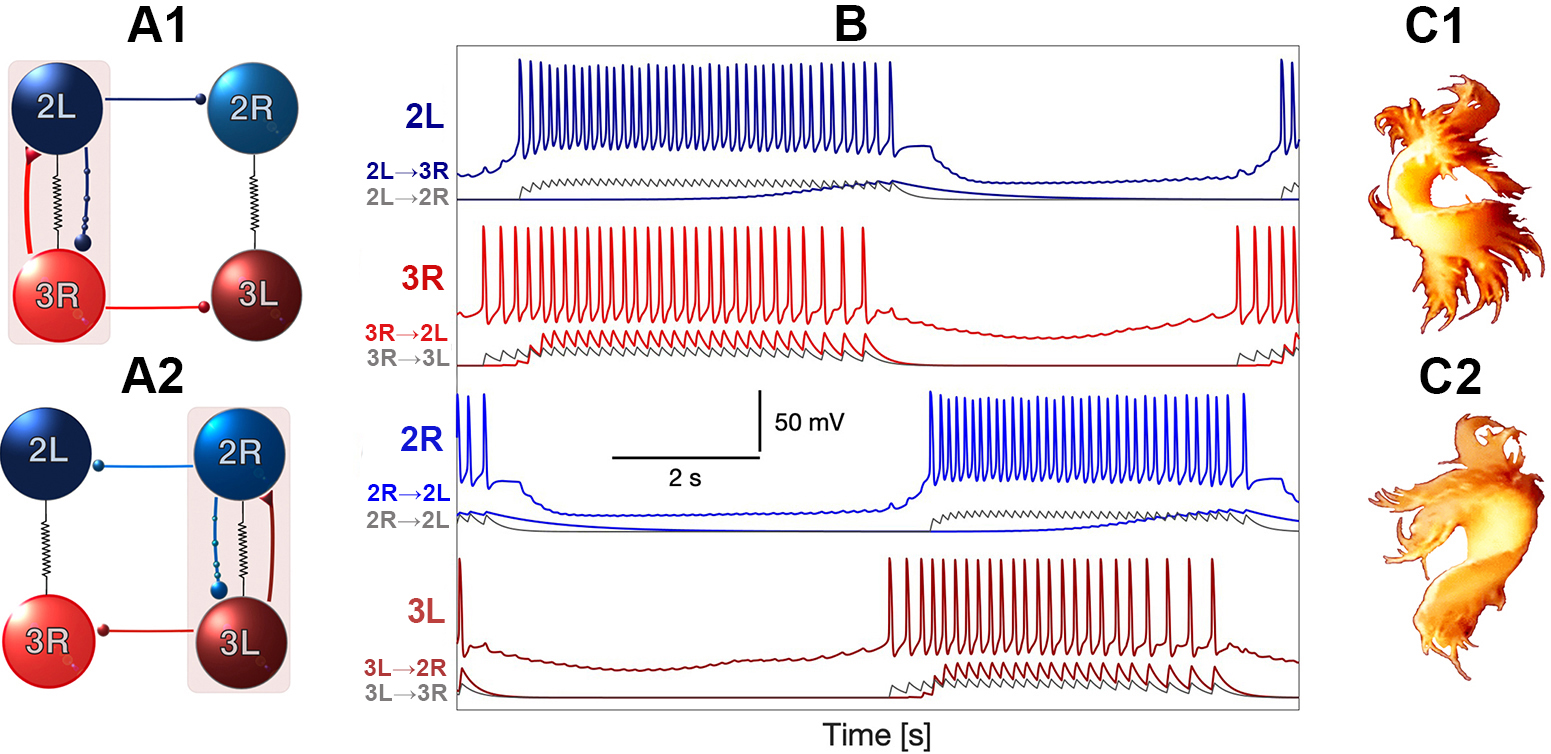
\includegraphics[width=\textwidth]{fig1.jpg}
\caption{{\bf Mechanism of left--right alternation: two reciprocally inhibitory E/I sub-networks generate anti-phase bursting.}
(A1--A2) Schematic of the contralateral E/I modules (Si3R$\leftrightarrows$Si2L and Si3L$\leftrightarrows$Si2R) embedded within reciprocally inhibitory half-center oscillators (Si3R$\leftrightarrows$Si3L below and Si2R$\leftrightarrows$Si2L above) that enforce bilateral alternation.
In A1 the right module (Si3R$\to$Si2L) is active while the left module is suppressed; in A2 the roles are reversed.
When isolated, each E/I module is tuned to be ``almost-oscillatory''---exhibiting damped oscillations or subthreshold rhythmic fluctuations rather than sustained limit cycles---so that network coupling is required to recruit them into coordinated bursting.
(B) Corresponding model voltage traces (thick colored) and simulated neurotransmitter release probabilities (thin curves): the top two traces show Si2L and Si2R, while the bottom two traces show Si3L and Si3R.
Red denotes excitatory Si3$\to$Si2 logistic synapses with faster kinetics, grey reciprocal inhibitory $\alpha$-synapses within the Si3 and within the Si2 pairs, and blue the slower logistic Si2$\to$Si3 inhibition that terminates each burst and sets episode duration.
(C1--C2) Sketch of corresponding whole-body undulations for consecutive left--right episodes.}
\label{fig:ei_mechanism}
\end{figure}

%%% Figure 2: Synaptic timescales (fig2.jpg)
\begin{figure}[htbp]
\centering

\includegraphics[width=\textwidth]{fig2.jpg}
\caption{{\bf Synaptic timescales in the model match experimental recordings.}
Compare panels~C and~D with the corresponding neurophysiological recordings presented in Fig.~7 of Sakurai \& Katz (2022).
(A--B) Three positive current pulses of progressively increasing amplitude applied to Si2R produce graded inhibitory postsynaptic potential (IPSP) responses in the contralateral Si2L, demonstrating the amplitude scaling of reciprocal inhibition.
(C--D) Two current pulses injected into Si2R evoke accumulating IPSP responses in Si2L and elicit dual-timescale responses in Si3L: a fast depolarizing component mediated by electrical coupling, followed by slower inhibition mediated by the logistic synapse.
The temporal separation between these components---tens of milliseconds for electrical coupling versus hundreds of milliseconds for chemical inhibition---matches the experimentally observed dynamics and establishes the timescales that govern burst shaping.}
\label{fig:synaptic_timescales}
\end{figure}

%%% Figure 3: CPG Assembly (fig3.jpg)
\begin{figure}[htbp]
\centering
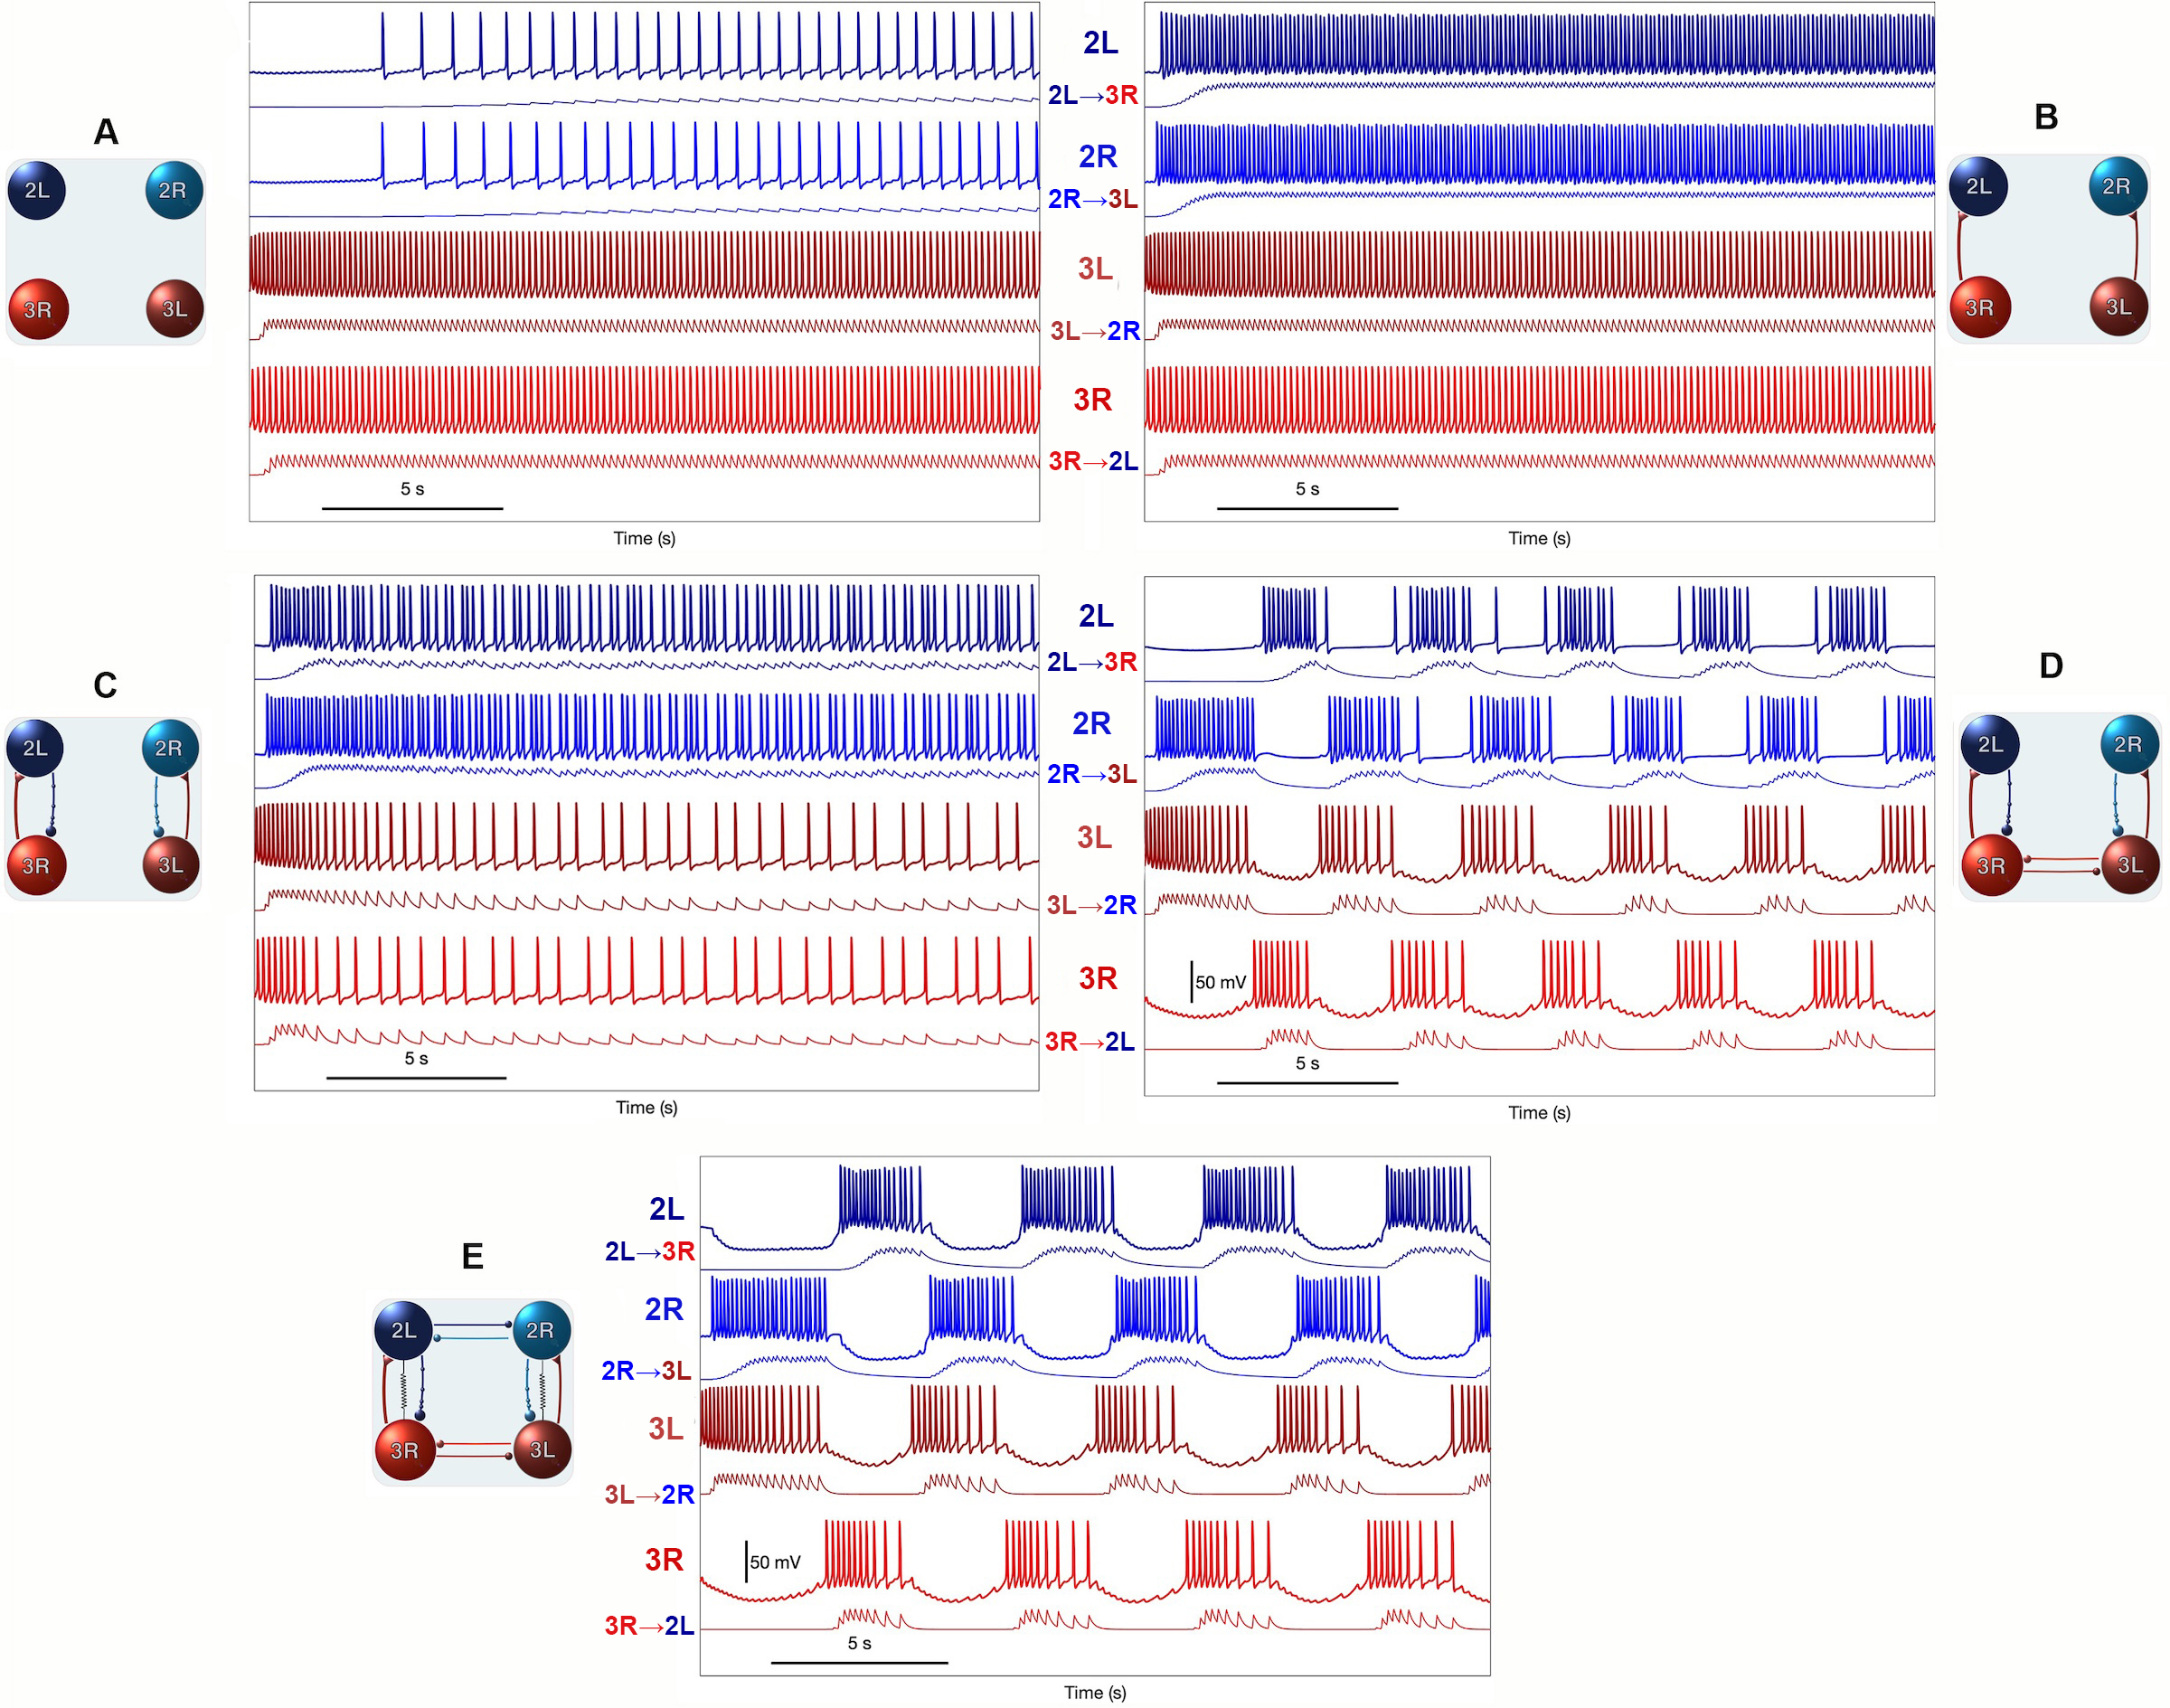
\includegraphics[width=\textwidth]{fig3.jpg}
\caption{{\bf CPG assembly in five sequential steps.}
(A) Four uncoupled interneurons, with Si3 neurons exhibiting intrinsic excitability and firing at a higher rate.
(B) Si3 neurons provide fast excitatory drive to contralateral Si2 neurons.
(C) Si2 neurons deliver slow inhibitory feedback to Si3 neurons to slow them down.
(D) Reciprocal inhibition between contralateral Si3 neurons triggers an initial rhythm formation.
(E) Reciprocally inhibitory synapses activated between contralateral Si2 neurons, along with two electrical synapses between Si3R$\leftrightarrows$Si2L and Si3L$\leftrightarrows$Si2R pairs of interneurons, generate stably the network-level bursting in the swim CPG model of \textit{Dendronotus iris}.
The traces underneath the voltage waveforms represent the corresponding neurotransmitter probability $s(t)$ in the pre-synaptic neurons.}
\label{fig:assembly}
\end{figure}

%%% Figure 4: Model vs experimental comparison (fig4.jpg)
\begin{figure}[htbp]
\centering

\includegraphics[width=\textwidth]{fig4.jpg}
\caption{{\bf Model responses to targeted perturbations match experimental recordings.}
Each panel shows model traces (top) alongside corresponding experimental recordings from Sakurai \& Katz (2016) (bottom).
(A) Depolarization of Si2L: injecting positive current into Si2L disrupts the ongoing rhythm; upon current removal, the network rapidly recovers coordinated bursting.
(B) Hyperpolarization of Si2L: injecting negative current into Si2L silences this neuron while the contralateral neurons continue oscillating; the network resumes normal activity upon release.}
\label{fig:perturbation_responses}
\end{figure}

%%% Figure 5: Si1 control and neuromodulation (fig5.jpg)
\begin{figure}[htbp]
\centering
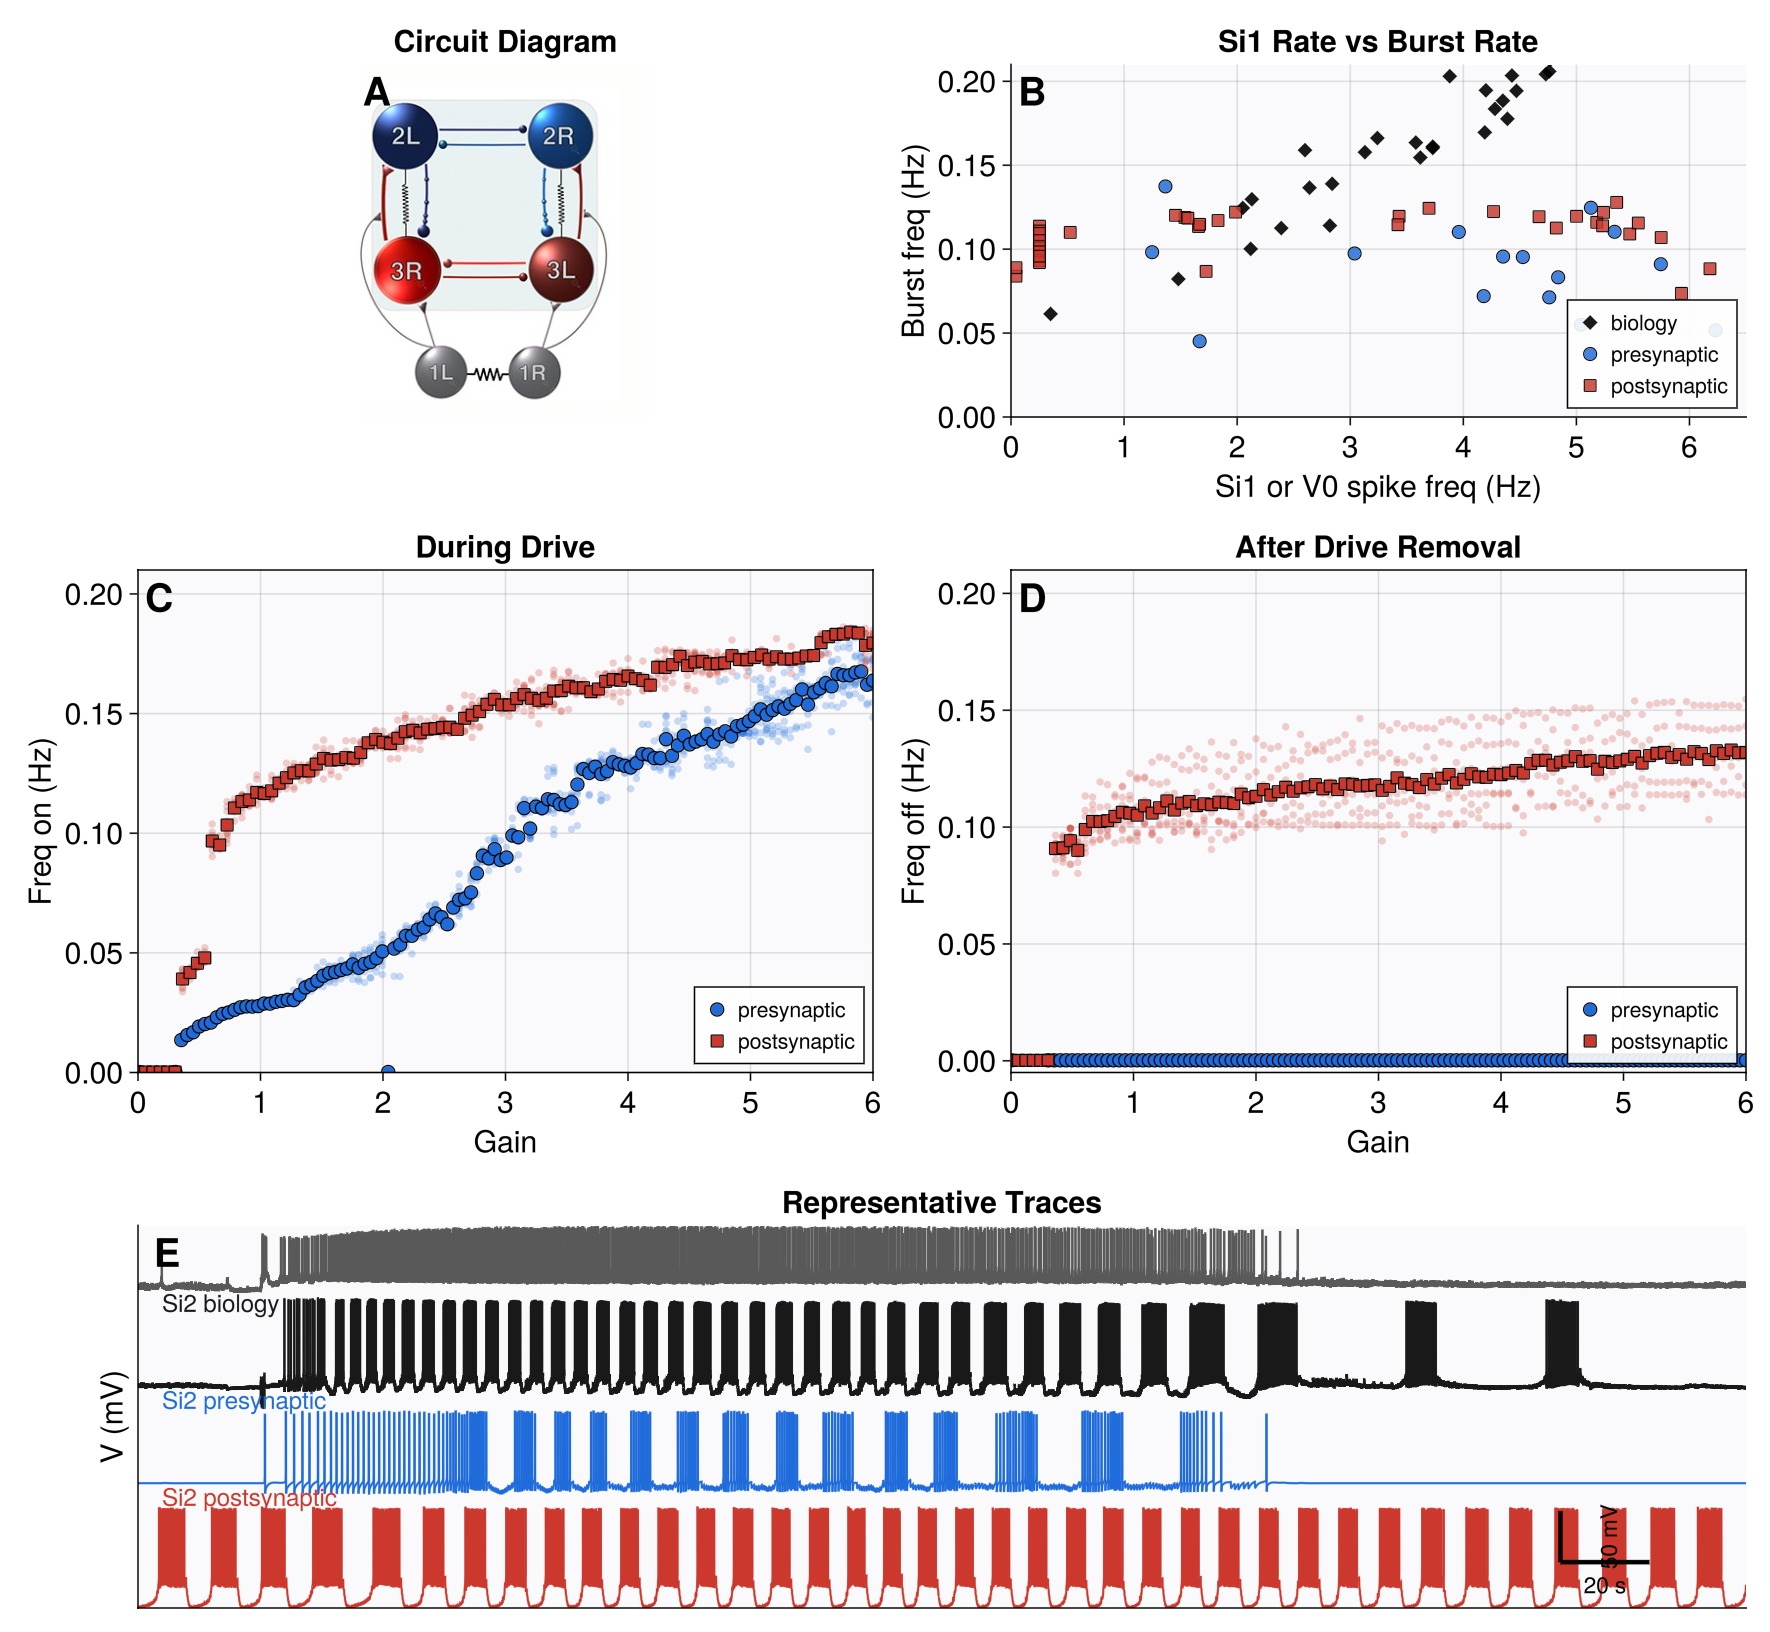
\includegraphics[width=\textwidth]{fig5.jpg}
\caption{{\bf Si1-dependent modulation of the Si3$\to$Si2 pathway regulates burst frequency during sustained drive.}
(A) Schematic of the five-cell swim circuit highlighting direct Si1 excitation of Si3 neurons and activity-dependent modulation of the Si3$\to$Si2 excitatory pathway.
(B) Relationship between Si1 spike rate and burst frequency.
Grey circles and grey fit line show digitized points from the published biological summary in Sakurai \& Katz (2019) \cite{sakurai2019command}, black triangles and black fit line show measurements extracted directly from the representative biological Si1/Si2 trace pair, and blue circles and red squares show matched model measurements from representative presynaptic and postsynaptic simulations, respectively.
(C) Scan of the dimensionless modulatory gain parameter $g_m$ during sustained drive.
In the presynaptic condition, gain multiplies the logistic Si3$\to$Si2 accumulation-rate parameter $\alpha$; in the postsynaptic condition, the same gain multiplies the effective synaptic conductance.
Both scans show gain-dependent changes in burst frequency, with different response curves for the two modulation targets.
Faint points show individual measured intervals; saturated markers show gain-wise means.
(D) Representative biological and model traces.
Top two traces show the biological Si1 and Si2 recordings.
Blue and red traces show the corresponding Si2 activity produced by presynaptic and postsynaptic model variants under the same Si1 drive, and the purple trace shows the shared modulatory variable $s_m$.
Triangles, circles, and squares mark detected burst onsets from the biological, presynaptic, and postsynaptic traces, respectively, and these onset-to-onset intervals are the measurements used for the rate-matching analysis in panel B.
The scale bar in panel D denotes 20~s and 50~mV.}
\label{fig:si1_neuromod}
\end{figure}

%%% Figure 6: Summary / Conclusion (fig6.jpg)
\begin{figure}[htbp]
\centering
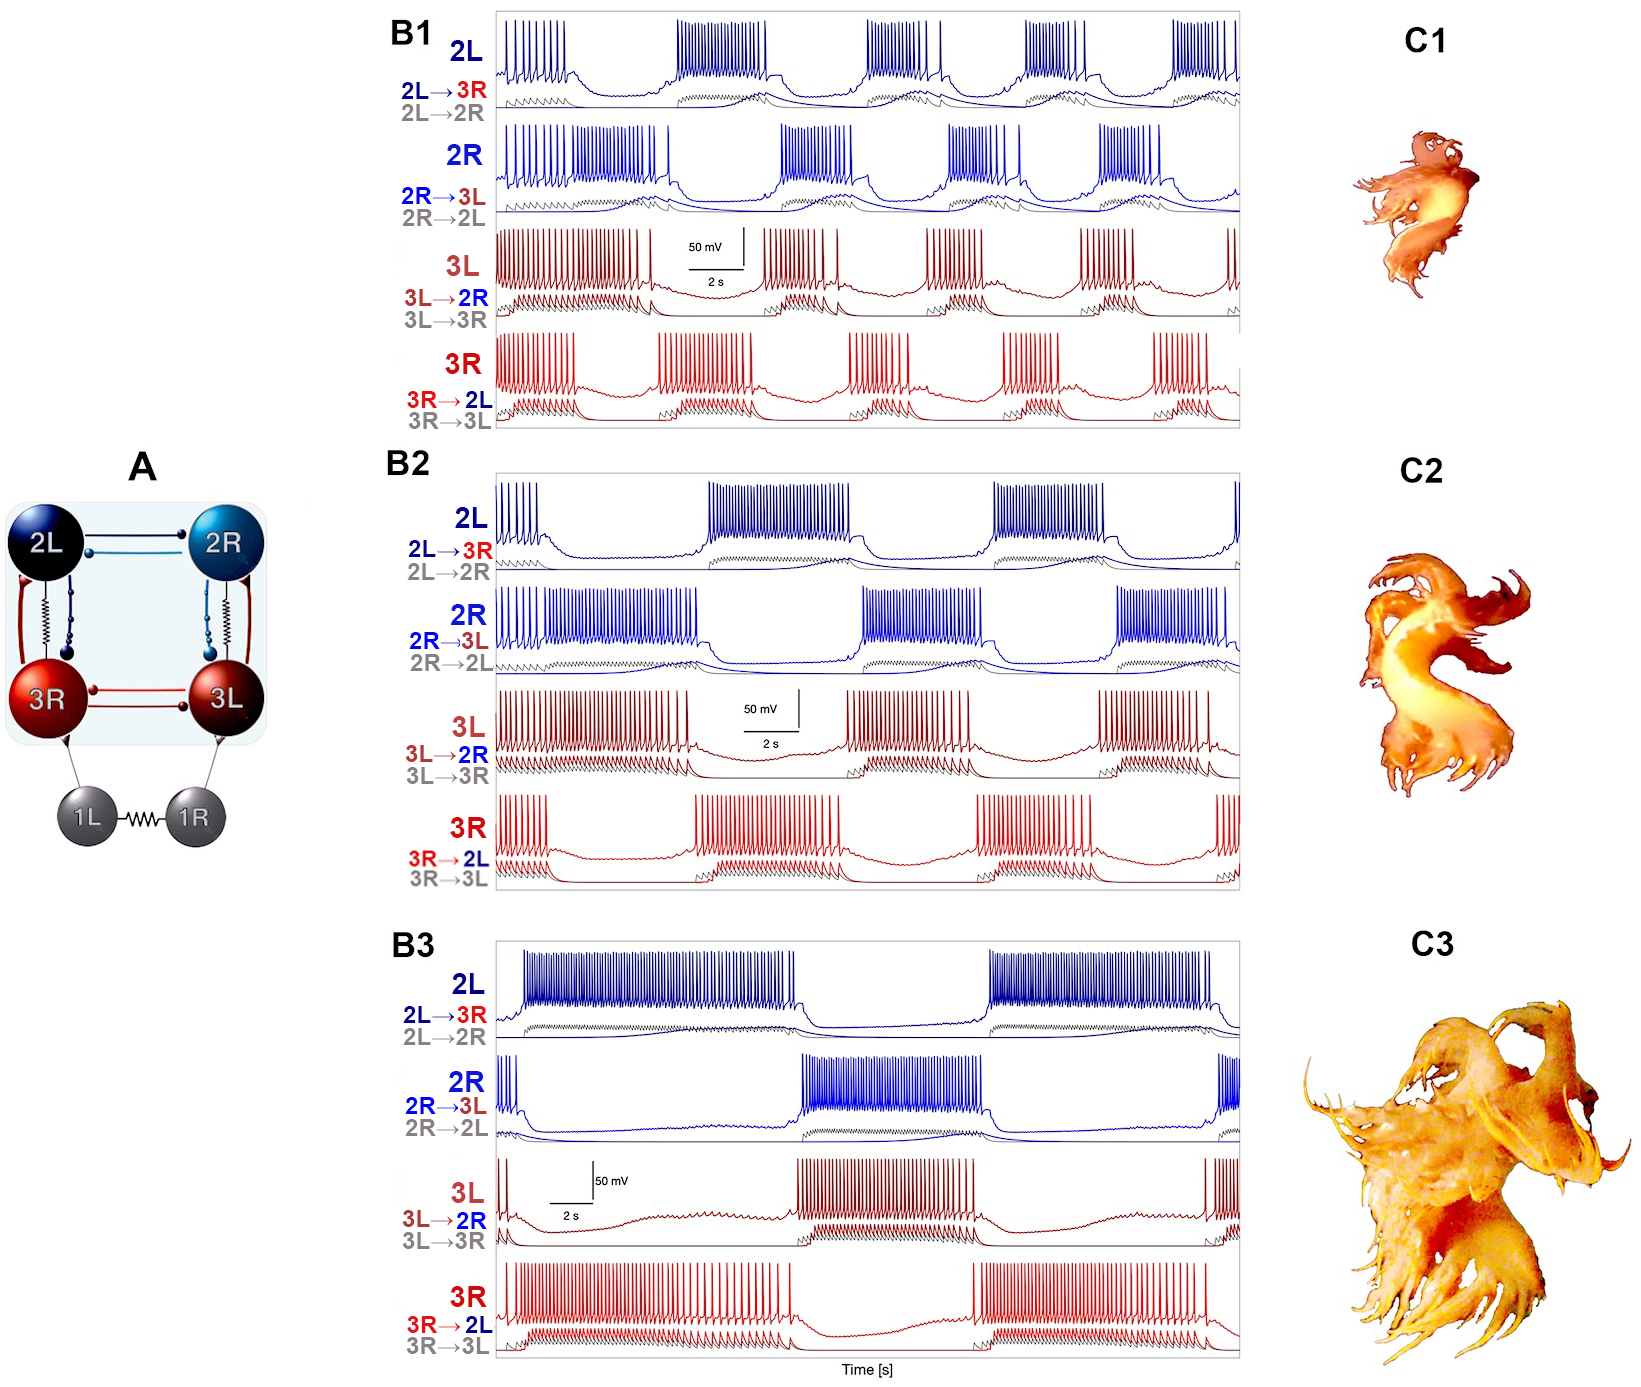
\includegraphics[width=\textwidth]{fig6.jpg}
\caption{{\bf Circuit architecture and burst frequency adaptability in the \textit{Dendronotus iris} swim CPG.}
The four-cell circuit assembles excitatory--inhibitory loops together with two contralateral half-center oscillators into a network that reliably produces left--right alternating bursts.
(A) Schematic of the canonical swim CPG circuitry composed of the four core interneurons---Si2L/R and Si3L/R---organized into two bilaterally symmetric E/I modules.
(B1--B3) Representative model traces showing voltage waveforms at three different burst frequencies, demonstrating the range of rhythmic output the network can produce.
(C1--C3) Conceptual illustration of how burst frequency modulation could accommodate variation in body size.}
\label{fig:summary}
\end{figure}

\newpage
\section*{SUPPLEMENTAL FIGURE LEGENDS}

%%% Figure S1: Additional perturbations (figS1.jpg)
\begin{figure}[htbp]
\centering
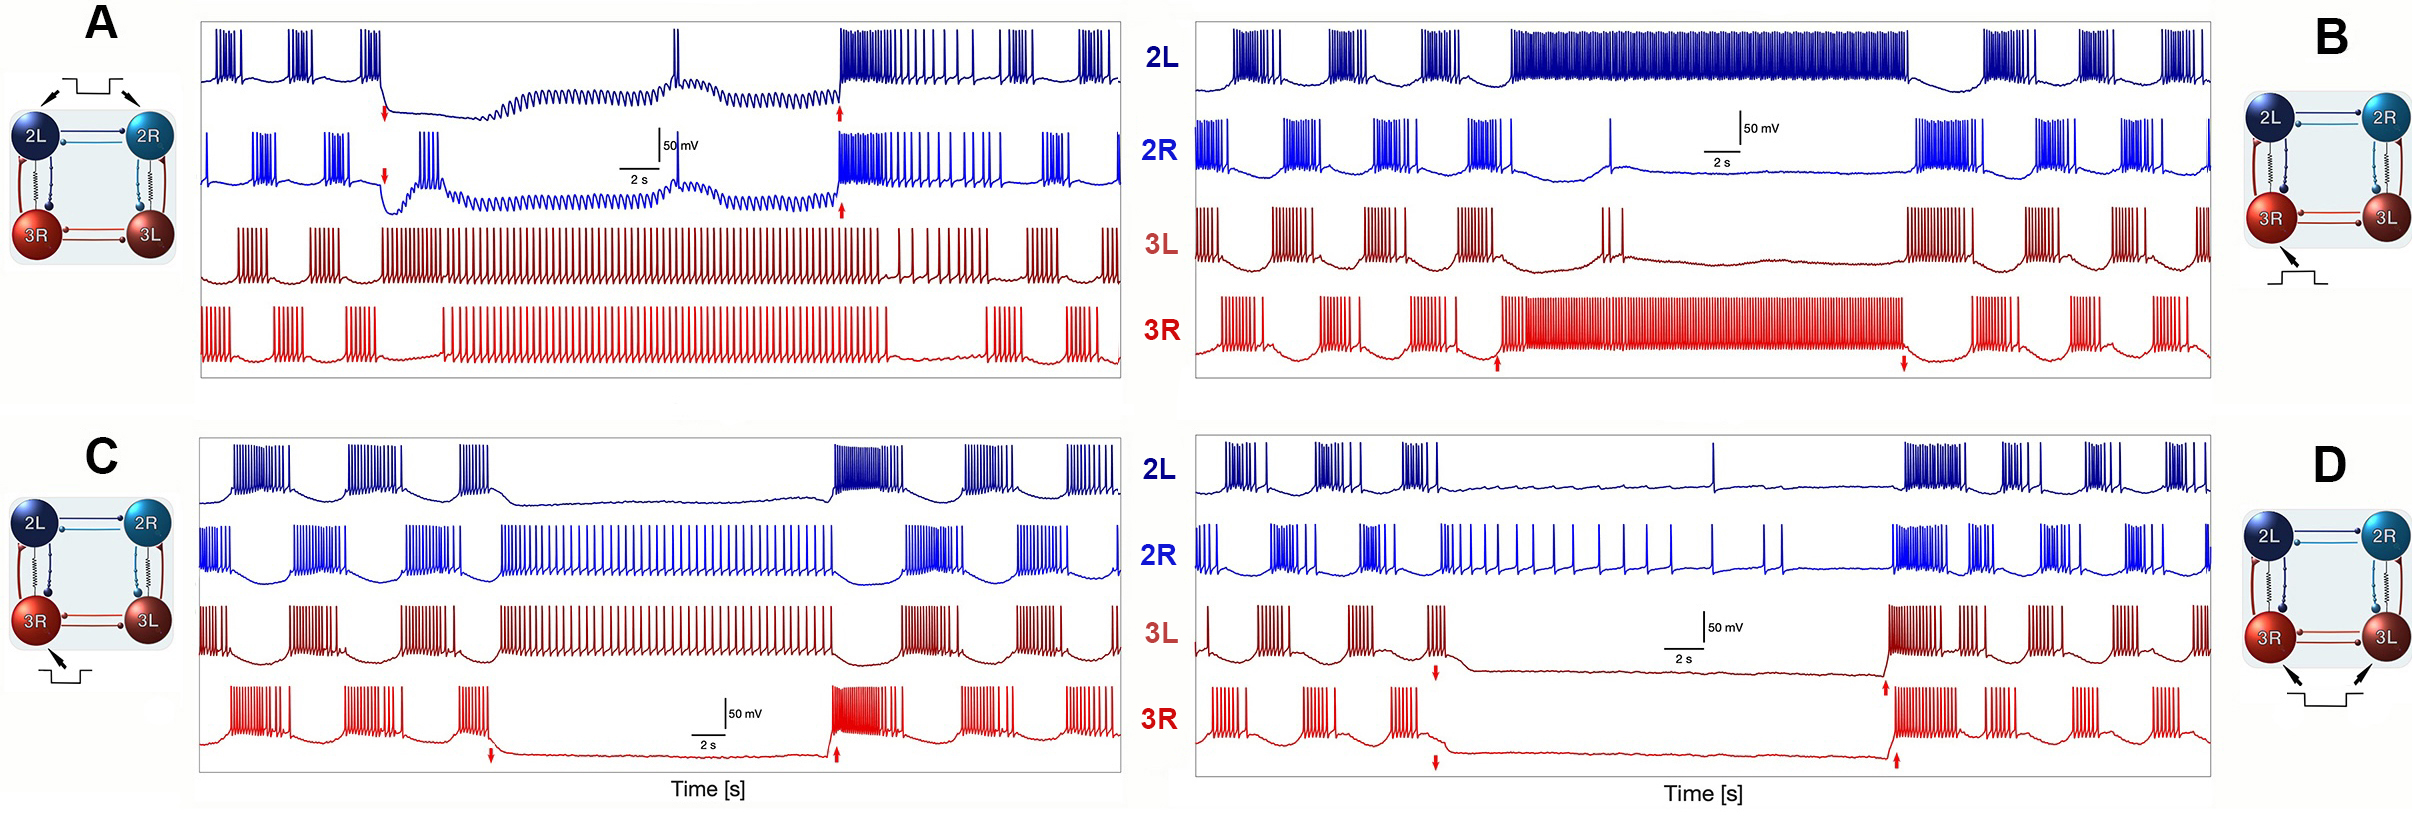
\includegraphics[width=\textwidth]{figS1.jpg}
\caption{{\bf Additional targeted perturbation experiments.}
Model responses to perturbations corresponding to Figs.~5C and E--G of Sakurai \& Katz (2016).
(A) Bilateral hyperpolarization of both Si2 neurons; the network recovers but restoration takes longer than unilateral cases.
(B) Positive current pulse to Si3R forces sustained high-frequency spiking; circuit rapidly returns to antiphase rhythm upon pulse termination.
(C) Hyperpolarizing Si3R silences it and its electrical partner Si2L.
(D) Bilateral hyperpolarization of both Si3 neurons completely abolishes network activity; rapid restoration upon pulse removal.}
\label{fig:supp_perturbations}
\end{figure}

%%% Figure S2: Symmetric perturbations (figS2.jpg)
\begin{figure}[htbp]
\centering
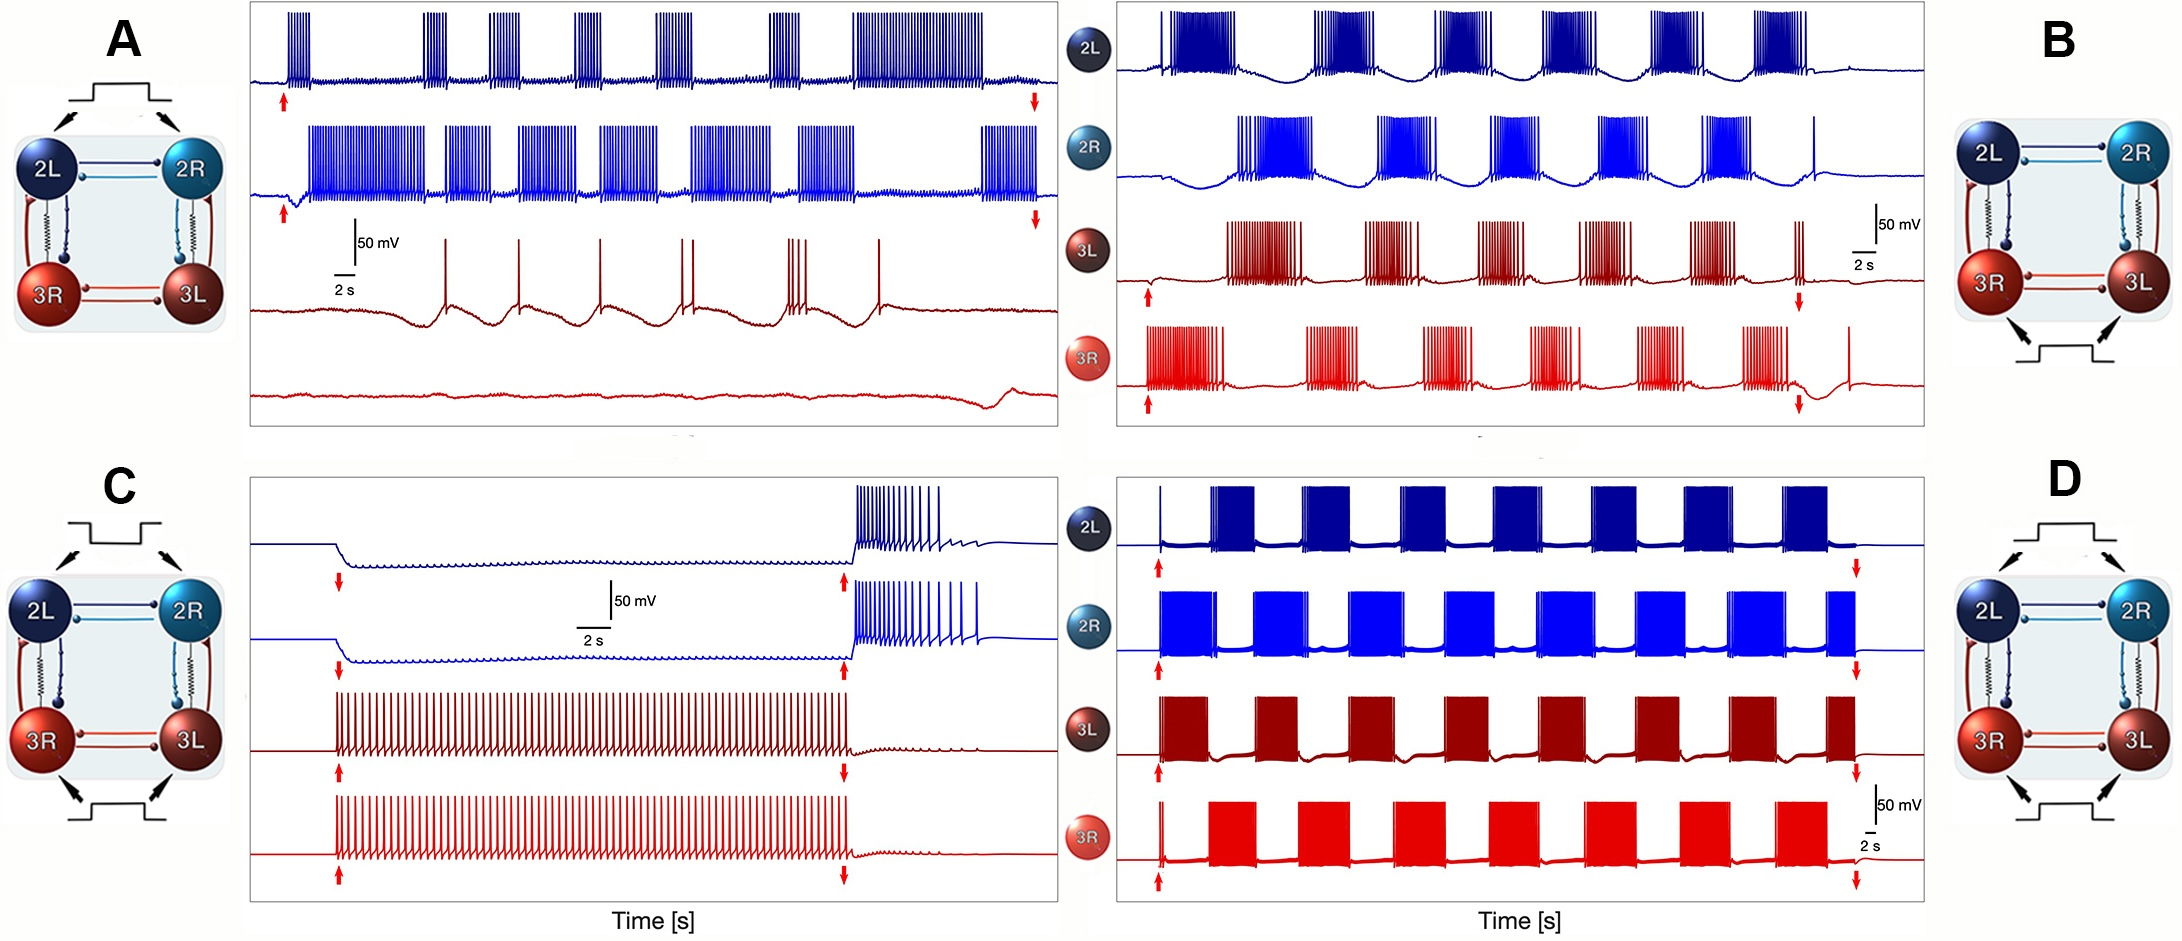
\includegraphics[width=\textwidth]{figS2.jpg}
\caption{{\bf Symmetric perturbation experiments.}
Model responses to bilateral depolarization corresponding to Fig.~7 of Sakurai \& Katz (2016).
(A--B) Bilateral depolarization of both Si2 neurons: simultaneous positive current injection into Si2L and Si2R produces coordinated high-frequency activity.
(C--D) Bilateral depolarization of both Si3 neurons: simultaneous positive current injection into Si3L and Si3R produces sustained network excitation.}
\label{fig:supp_symmetric}
\end{figure}


\newpage

%%% References
\bibliography{references}

\newpage

%%% STAR Methods
\section*{STAR METHODS}

%%% Key Resources Table
\subsection*{Key resources table}

\begin{tabular}{|l|l|l|}
\hline
\textbf{REAGENT or RESOURCE} & \textbf{SOURCE} & \textbf{IDENTIFIER} \\
\hline
\multicolumn{3}{|l|}{\textbf{Software and algorithms}} \\
\hline
MATLAB & MathWorks & https://www.mathworks.com/products/matlab \\
\hline
Custom simulation code & This paper & https://github.com/jamesjscully/Dendronotus \\
\hline
\end{tabular}


%%% Method Details
\subsection*{Method details}

\subsubsection*{Neuron model}

The dynamics of the membrane potential, $V$, is governed by the following equation:
\begin{equation}
 	C_{m} {V}^\prime = -I_{I} - I_K - I_{T}  - I_{KCa} -  I_{h}  - I_{leak}  - I_{syn},
\end{equation}
where $C_m = 1$\,nF is the membrane capacitance.

The fast inward sodium and calcium $I_{I}$-current is given by
\begin{equation}
I_{I}=g_{I}\,h\, m^{3}_{\infty}(V)(V-E_{I}),
\end{equation}
with the reversal potential $E_{I}=30$mV and the maximal conductance value $g_{I}=4$nS, and where the infinite functions are given by
\begin{align}
 m_{\infty}(V) &= \frac{\alpha_{m}(V)}{\alpha_{m}(V) +\beta_{m}(V)},   \\
 \alpha_{m}(V) &= 0.1 \frac{50-V_s}{-1+e^{(50-V_s)/10}}, \\
 \beta_{m}(V) &= 4 e^{(25-V_s)/18}.
\end{align}

The dynamics of its inactivation gating variable $h$ is given by
\begin{align}
 {h}^\prime &=  \frac{h_{\infty}(V)-h}{ {\tau_{h}(V)} }, \\
h_{\infty}(V) &= \frac{\alpha_{h}(V)}{\alpha_{h}(V) +\beta_{h}(V)}, \\
 \tau_{h}(V) &= \frac{12.5}{\alpha_{h}(V) +\beta_{h}(V)},
\end{align}
where
\begin{align}
 \alpha_{h}(V) &= 0.07 e^{(25-V_s)/20}, \\
 \beta_{h}(V) &= \frac{1}{1+e^{(55-V_s)/10}}, \\
 V_s &= \frac{127V+8265}{105}{\rm mV}.
\end{align}

The fast potassium $I_K$-current is given by the equation
\begin{equation}
I_K=g_{K} n^{4}(V-E_{K}),
\end{equation}
with the reversal potential $E_{K}=-75$mV and the maximal conductance set as $g_K=0.3$nS.
The dynamics of inactivation gating variable are described by
\begin{align}
{n}^\prime &= \frac{n_{\infty}(V)-n}{\tau_{n}(V)}, \\
n_{\infty}(V) &= \frac{\alpha_{n}(V)}{\alpha_{n}(V) +\beta_{n}(V)}, \\
\tau_{n}(V) &= \frac{12.5}{\alpha_{n}(V) +\beta_{n}(V)}, \\
\alpha_{n}(V) &= 0.01 \frac{55-V_s}{e^{(55-V_s)/10}-1}, \\
\beta_{n}(V) &= 0.125 e^{(45-V_s)/80}.
\end{align}

The rapidly depolarizing h-current is given by
\begin{equation}
I_{h}=g_{h} \frac{y (V-E_{h})}{(1+e^{-(V-63)/7.8})^3},
\end{equation}
with $E_{h}=70$mV, and $g_h=0.0006$nS; the dynamics of its $y$-activation probability is described by
\begin{equation}
{y}^\prime = \frac{1}{2} \left [ \frac{1}{1+e^{10(V-50)}}-y \right ]/ \left [ 7.1+\frac{10.4}{1+e^{(V+68)/2.2}} \right ].
\end{equation}

The leak current is given by
\begin{equation}
I_{leak} =g_{L} (V-E_{L}),
\end{equation}
with $E_{L} =-40{\rm mV}$, and $g_{L}=0.003{\rm nS}$.

The sub-group of slow currents in the model includes the TTX-resistant sodium and calcium $I_{T}$-current given by
\begin{equation}
 I_{T} = g_{T} x (V-E_{I}),
\end{equation}
with $E_{I} =30{\rm mV}$ and $g_{T}=0.01{\rm nS}$, where the dynamics of its slow activation variable are described by
\begin{align}
{x}^\prime &= \frac{x_{\infty}(V)-x}{\tau_{x}}, \\
x_{\infty} &= \frac{1}{1+e^{-0.15(V+50-\Delta_x)}},
\end{align}
with the time constant $\tau_{x} = 100$\,ms.

The slowest outward ${\rm Ca}^{2+}$ activated $K^+$ current given by
\begin{equation}
I_{KCa} =g_{KCa}\frac{[\rm Ca]_i}{0.5+[\rm Ca]_i}(V-E_{K}),
\end{equation}
with $E_{K}=-75\mbox{mV}$, and $g_{KCa}=0.03$, where the dynamics of intracellular calcium concentration is governed by
\begin{equation}
{[\rm Ca]}^\prime  =  \rho \left ( K_{c}\, x\, (E_{\rm Ca}-V + \Delta_{\rm Ca})-[\rm Ca] \right  )
\end{equation}
with the Nernst reversal potential $E_{Ca}=140$mV, and small constants $\rho= 0.0003{\rm ms}^{-1}$ and $K_c=0.0085{\rm mV}^{-1}$.


\subsubsection*{Synapse models}

\paragraph{Fast $\alpha$-synapses.}
Fast excitatory and inhibitory synapses are modeled using the $\alpha$-synapse formalism \cite{destexhe1994synthesis, destexhe1998kinetic, Rall67}.
The synaptic current is given by
\begin{equation}
I_{syn} = g_{syn} \cdot s \cdot (V_{post} - E_{syn}),
\end{equation}
where $g_{syn}$ is the maximal synaptic conductance, $s$ is the synaptic gating variable, and $E_{syn}$ is the reversal potential ($E_{syn} = +40$mV for excitation, $E_{syn} = -80$mV for inhibition).

The synaptic gating variable $s$ follows
\begin{align}
{s}^\prime &= \alpha \cdot f_{\infty}(V_{pre}) \cdot (1 - s) - \beta \cdot s,
\end{align}
where $f_{\infty}(V_{pre})$ is a sigmoid function of presynaptic voltage:
\begin{equation}
f_{\infty}(V_{pre}) = \frac{1}{1 + e^{-k(V_{pre} - V_{th})}},
\end{equation}
with threshold $V_{th} = -20$\,mV and slope $k = 20$\,mV$^{-1}$.

\paragraph{Logistic synapses.}
The contralateral E/I module synapses (both Si3$\to$Si2 excitation and Si2$\to$Si3 inhibition) use a novel logistic synapse model that captures synaptic accumulation dynamics:
\begin{equation}
{s}^\prime = \alpha \cdot s \cdot (1-s) \cdot f_{\infty}(V_{pre}) - \beta \cdot (s - s_0),
\end{equation}
where $f_{\infty}(V_{pre})$ is the same sigmoid function of presynaptic voltage, and $s_0 \ll 1$ is a baseline release rate.
The key difference from the standard $\alpha$-synapse is the $s(1-s)$ term, which creates logistic growth dynamics: the synapse accumulates slowly when $s$ is small, reaches maximal accumulation rate at $s = 0.5$, and saturates as $s$ approaches 1.
The Si2$\to$Si3 inhibitory synapses use slower kinetics ($\alpha = 0.012$\,ms$^{-1}$) that produce summation on timescales of hundreds of milliseconds, setting the burst period.
The Si3$\to$Si2 excitatory synapses use faster kinetics ($\alpha = 0.05$\,ms$^{-1}$) but retain the logistic accumulation dynamics for consistent E/I module behavior.

\paragraph{Synaptic normalization.}
Without normalization, the synaptic gating variable $s$ is bounded between 0 and a maximum value that depends on the kinetic parameters $\alpha$ and $\beta$.
Since the synaptic conductance is proportional to $g_{syn} \cdot s$, changing $\alpha$ and $\beta$ would inadvertently affect the effective synaptic strength, creating unwanted codependencies between kinetic timescales and synaptic amplitude.
To decouple synaptic strength from kinetic parameters, we normalize the synaptic current:
\begin{equation}
I_{syn} = g_{syn} \cdot \frac{s}{\text{scale}_s} \cdot (V_{post} - E_{syn}),
\end{equation}
where the scaling factors depend on synapse type:
\begin{align}
\text{scale}_{\text{fast}} &= \frac{\alpha}{\alpha + \beta} \quad \text{(for $\alpha$-synapses)}, \\
\text{scale}_{\text{slow}} &= \frac{\alpha - \beta}{\alpha} \quad \text{(for logistic synapses)}.
\end{align}
These factors normalize the theoretical asymptotic limit to unity for all parameter combinations, ensuring that $g_{syn}$ directly represents the maximum synaptic conductance independent of the kinetic parameters.


\subsubsection*{Network connectivity}

The \textit{Dendronotus iris} swim CPG model consists of four core interneurons (Si2L, Si2R, Si3L, Si3R) with the following synaptic connections:
\begin{itemize}
    \item \textbf{Contralateral excitation}: Si3R$\to$Si2L and Si3L$\to$Si2R (logistic synapses)
    \item \textbf{Contralateral inhibition}: Si2L$\to$Si3R and Si2R$\to$Si3L (logistic synapses)
    \item \textbf{Reciprocal Si3 inhibition}: Si3L$\longleftrightarrow$Si3R ($\alpha$-synapses)
    \item \textbf{Reciprocal Si2 inhibition}: Si2L$\longleftrightarrow$Si2R ($\alpha$-synapses)
    \item \textbf{Electrical coupling}: Si3R$\longleftrightarrow$Si2L and Si3L$\longleftrightarrow$Si2R (gap junctions)
\end{itemize}

The command neuron Si1 provides neuromodulatory input that scales the effective strength of Si3$\to$Si2 excitation, enabling frequency control.


\subsubsection*{Network assembly and calibration}

We assembled the four-cell swim CPG network by integrating validated two-cell subnetworks---specifically half-center oscillators (HCOs) and excitatory-inhibitory (E/I) modules---following the approach in \cite{scully2024pairing}.
Synaptic kinetics for mutual inhibition and E/I interactions were matched to previously characterized modules.

Cellular parameters were preserved from prior models, with the exception of Si3 neurons, whose endogenous excitability was increased by shifting the voltage threshold $\Delta[\text{Ca}]$ by 5\,mV to promote spiking.

\paragraph{Almost-oscillatory sub-circuits.}
By ``almost-oscillatory'' sub-circuits, we mean configurations that exhibit damped oscillatory behavior or subthreshold rhythmic fluctuations when isolated, but do not sustain stable limit-cycle oscillations without network interactions.
These sub-circuits lie close to oscillatory regimes in parameter space, near bifurcations that separate quiescent from rhythmic states, such that modest network coupling can recruit them into coordinated bursting.
This design principle contrasts with CPG architectures built from intrinsically bursting pacemaker neurons that generate robust oscillations independently of network context.

\paragraph{Calibration protocol.}
Network calibration was performed by symmetrically tuning synaptic conductances using the following protocol:
\begin{enumerate}
    \item \textbf{Configuration:} Pre- and postsynaptic voltage variables were assigned according to the known swim circuits of \textit{Dendronotus iris} \cite{SakuraiKatz2016}.
    \item \textbf{Initialization:} All cells were set to a quiescent state with synaptic conductances at zero.
    \item \textbf{Drive:} Synaptic drive was applied to Si3 until the excitatory postsynaptic gating variable $s$ showed sustained accumulation, measured by local minima rising above 0.1 and saturating over 0.5--3\,s.
    \item \textbf{Excitation:} Excitatory conductance from Si3 to contralateral Si2 was increased until inhibitory $s$ (Si2-to-Si2) reached minima above 0.1 over 0.5--3\,s.
    \item \textbf{Slow inhibition:} Inhibitory conductance in the E/I pair was raised until Si3 frequency decreased by 50\% over 1\,s.
    \item \textbf{Fast inhibition:} Inhibitory conductances for both HCOs (Si2L--Si2R and Si3L--Si3R) were elevated until a stable burst rhythm emerged, visually matching empirical voltage traces \cite{SakuraiKatz2016}.
    \item \textbf{Fine-tuning:} Excitability was adjusted slightly (e.g., $\Delta[\text{Ca}] < 2$\,mV) to achieve a duty cycle matching experimental observations.
\end{enumerate}


\subsubsection*{Model validation}

To validate the CPG model, we performed direct current injection into the voltage equation of selected interneurons, adding a current term to the right-hand side of the membrane potential equation and varying its amplitude to mimic experimental perturbations.
No additional parameter tuning, optimization, or fitting procedures were employed during these tests.
This approach ensures that the model's responses reflect its intrinsic dynamics and structure, maintaining the integrity of the validation process.

All validation responses shown are typical: simulations use random initial conditions for the four interneurons and synapses, plus calibrated colored noise (up to 20 Hz), to probe robustness.
This explains trial-to-trial variability in initial phase and demonstrates that the model's behavior is not dependent on specific initial conditions.

Validation focuses on qualitative reproduction of experimental phenomena through systematic comparison of model output with published voltage traces and perturbation responses \cite{SakuraiKatz2016, sakurai2019command, sakurai2022bursting}.
Quantitative parameter fitting was not attempted due to limited availability of quantitative measurements in the experimental literature.
Our approach prioritizes mechanistic insight---demonstrating that the proposed circuit architecture and synaptic dynamics can reproduce the diversity of observed behaviors---over numerical precision in matching specific parameter values.


\subsubsection*{Neuromodulation}

Si1 neurons modulate the Si3$\to$Si2 excitatory synapses through a dynamic modulatory variable $s_m \in [0, 1]$ that evolves according to
\begin{equation}
{s_m}^\prime = \alpha_m \cdot s_m \cdot (1 - s_m) \cdot f_{\infty}(V_{Si1}) - \beta_m \cdot (s_m - s_{m}^0),
\end{equation}
where $f_{\infty}(V_{Si1})$ is the sigmoid function of the Si1 presynaptic voltage, and $0 < s_m^0 \ll 1$ is a baseline value.

In the MATLAB implementation, modulation is normalized by
\begin{equation}
\text{scale}_m = \frac{\alpha_m - \beta_m}{\alpha_m},
\end{equation}
and the gain parameter $g_m$ enters through the factor $(1 + g_m s_m / \text{scale}_m)$.
When $s_m = 0$, the synapse operates at baseline strength.
We compare two modulatory mechanisms that target distinct biophysical processes:

\paragraph{Postsynaptic modulation.}
The modulatory variable scales the maximal conductance of the logistic Si3$\to$Si2 synapse directly:
\begin{equation}
I_{syn} = g_{syn} \cdot \left(1 + g_m \frac{s_m}{\text{scale}_m}\right) \cdot \frac{s}{\text{scale}_s} \cdot (V_{post} - E_{syn}),
\end{equation}
We term this ``postsynaptic'' because the synaptic conductance $g_{syn}$ characterizes the electrical properties of the postsynaptic membrane---specifically, the density and conductance of postsynaptic receptors and ion channels that determine the amplitude of the postsynaptic response.

\paragraph{Presynaptic modulation.}
Alternatively, the modulatory variable scales the accumulation rate $\alpha$ of the same logistic synapse:
\begin{equation}
{s}^\prime = \alpha \cdot \left(1 + g_m \frac{s_m}{\text{scale}_m}\right) \cdot s \cdot (1-s) \cdot f_{\infty}(V_{pre}) - \beta \cdot (s - s_0).
\end{equation}
We term this ``presynaptic'' because the gating variable $s(t)$ models the dynamics of neurotransmitter release, a process that occurs at the presynaptic terminal.
Modulating the $\alpha$ parameter affects the rate at which neurotransmitter accumulates, mimicking biological mechanisms such as changes in vesicle priming, calcium sensitivity, or release probability.

Both mechanisms increase effective synaptic strength, but presynaptic modulation additionally accelerates synaptic accumulation, producing qualitatively different effects on network dynamics as explored in the Results.

\subsubsection*{Neuromodulation scan and rate-matching procedure}

For the neuromodulation comparison in Fig.~\ref{fig:si1_neuromod}, we analyzed the circuit under sustained Si1 drive and compared two modulation targets within the Si3$\to$Si2 excitatory pathway.
In the presynaptic condition, the gain parameter multiplied the logistic accumulation-rate parameter $\alpha$.
In the postsynaptic condition, the same gain parameter multiplied the effective synaptic conductance.
For each condition, we scanned gain from 0 to 8 and measured burst frequency from successive Si2 burst intervals after excluding early transients.

To compare model output with experiment, we used the Si1 and Si2 traces digitized from preparation 130618-03 together with the published Si1-versus-burst summary data from Sakurai \& Katz (2019).
Burst onsets were detected from Si2 threshold crossings, and Si1 firing rate was computed within each inter-burst interval.
This produced paired measurements of Si1 spike frequency and burst frequency for both the biological traces and the representative model traces shown in Fig.~\ref{fig:si1_neuromod}E.
The same detection procedure was applied to both model variants.
For display and interval matching, the biological trace time base was stretched by a factor of 2 relative to the raw digitized recording; accordingly, frequencies extracted from the published summary points were divided by 2 so that the trace-based and summary-based biological comparisons were expressed on the same timescale.

\paragraph{Representative traces.}
The representative presynaptic and postsynaptic traces in Fig.~\ref{fig:si1_neuromod}E were generated by replaying the same digitized Si1 voltage trace into both model variants.
The representative presynaptic trace used control gain $g_m = 3.545$, chosen so that the modulated excitatory accumulation rate reached the cited target value under sustained drive.
The representative postsynaptic trace used control gain $g_m = 3.0$, together with conductance compensation in the unmodulated baseline, so that the effective excitatory conductance matched the cited target under the same saturated-drive assumption.

\paragraph{Figure-specific parameters.}
The clean neuromodulation dashboard figure was generated from the calibrated Julia analysis pipeline using the saved parameter set listed below.
These values define the exact scans and representative traces used for Fig.~\ref{fig:si1_neuromod} and should be taken as the figure-specific parameter source of truth for this analysis.

\begin{table}[htbp]
\centering
\caption{Figure 5 neuromodulation scan parameters}
\label{tab:neuromod_dashboard_params}
\begin{tabular}{|l|l|l|}
\hline
\textbf{Parameter} & \textbf{Value} & \textbf{Role in analysis} \\
\hline
$\Delta x_{\mathrm{Si2}}$ & $-4.0$ mV & Si2 slow-current voltage shift \\
$\Delta x_{\mathrm{Si3}}$ & $-4.0$ mV & Si3 slow-current voltage shift \\
$g_{0,\mathrm{pre}}$ & 0.0008 & Si1$\to$Si3 drive, presynaptic condition \\
$g_{0,\mathrm{post}}$ & 0.0016 & Si1$\to$Si3 drive, postsynaptic condition \\
$g_{m,\mathrm{pre}}^{\ast}$ & 3.545 & representative presynaptic trace gain \\
$g_{m,\mathrm{post}}^{\ast}$ & 3.0 & representative postsynaptic trace gain \\
$\alpha_1$ & 0.008 ms$^{-1}$ & Si1 synaptic activation rate \\
$\beta_1$ & 0.0016 ms$^{-1}$ & Si1 synaptic decay rate \\
$s_0^{\mathrm{floor}}$ & 0.013 & baseline Si1 synaptic floor \\
$\alpha_m$ & 0.006 ms$^{-1}$ & modulatory buildup rate \\
$\beta_m$ & $5.0\times10^{-5}$ ms$^{-1}$ & modulatory decay rate \\
$s_m^{\mathrm{floor}}$ & 0.0213 & baseline modulatory floor \\
$\Delta\mathrm{Ca}_{\mathrm{Si2}}$ & $-25.0$ mV & calcium shift, Si2 pair \\
$\Delta\mathrm{Ca}_{\mathrm{Si3}}$ & $-25.0$ mV & calcium shift, Si3 pair \\
$g_{\mathrm{base}}^{\mathrm{pre}}$ & 0.001 & baseline Si3$\to$Si2 conductance, presynaptic condition \\
$g_{\mathrm{base}}^{\mathrm{post}}$ & 0.04 & baseline Si3$\to$Si2 conductance, postsynaptic condition \\
$\alpha_{x,\mathrm{pre}}$ & 0.011 ms$^{-1}$ & baseline logistic accumulation, presynaptic condition \\
$\alpha_{x,\mathrm{post}}$ & 0.011 ms$^{-1}$ & baseline logistic accumulation, postsynaptic condition \\
$\beta_{x,\mathrm{pre}}$ & 0.001 ms$^{-1}$ & logistic decay, presynaptic condition \\
$\beta_{x,\mathrm{post}}$ & 0.001 ms$^{-1}$ & logistic decay, postsynaptic condition \\
$g_{\mathrm{inh,slow}}$ & 0.005 & Si2$\to$Si3 slow inhibition \\
$\alpha_{\mathrm{inh,slow}}$ & 0.015 ms$^{-1}$ & Si2$\to$Si3 inhibitory accumulation \\
$\beta_{\mathrm{inh,slow}}$ & 0.0005 ms$^{-1}$ & Si2$\to$Si3 inhibitory decay \\
$g_{\mathrm{Si2\leftrightarrow Si2}}$ & 0.0115 & reciprocal Si2 inhibition \\
$\alpha_{\mathrm{Si2\leftrightarrow Si2}}$ & 0.01 ms$^{-1}$ & reciprocal Si2 inhibitory rise \\
$\beta_{\mathrm{Si2\leftrightarrow Si2}}$ & 0.01 ms$^{-1}$ & reciprocal Si2 inhibitory decay \\
$g_{\mathrm{Si3\leftrightarrow Si3}}$ & 0.005 & reciprocal Si3 inhibition \\
$\alpha_{\mathrm{Si3\leftrightarrow Si3}}$ & 0.01 ms$^{-1}$ & reciprocal Si3 inhibitory rise \\
$\beta_{\mathrm{Si3\leftrightarrow Si3}}$ & 0.002 ms$^{-1}$ & reciprocal Si3 inhibitory decay \\
$t_1$ & 1000 ms & synaptic timescale parameter in the scan model \\
\hline
\end{tabular}
\end{table}


\subsubsection*{Simulation and analysis tools}

The core circuit-development and validation simulations were performed using custom MATLAB code.
For the neuromodulation dashboard analysis in Fig.~\ref{fig:si1_neuromod}, we used a Julia implementation of the same model equations to run parameter scans, generate representative traces, and extract matched Si1-rate versus burst-rate measurements.
Differential equations were integrated numerically with fixed trace sampling for visualization and burst detection.
Burst detection and period measurement were performed using threshold-crossing algorithms on the membrane voltage traces.


%%% Model Parameters
\subsection*{Model parameters}

Table~\ref{tab:intrinsic_params} lists intrinsic neuronal parameters, which are identical across all four interneurons except where noted.
Table~\ref{tab:synaptic_params} lists synaptic parameters for network connectivity.

\begin{table}[htbp]
\centering
\caption{Intrinsic neuronal parameters}
\label{tab:intrinsic_params}
\begin{tabular}{|l|l|l|l|}
\hline
\textbf{Parameter} & \textbf{Description} & \textbf{Value} & \textbf{Units} \\
\hline
\multicolumn{4}{|l|}{\textit{Fast inward current ($I_I$)}} \\
\hline
$g_I$ & Maximal conductance & 4 & nS \\
$E_I$ & Reversal potential & 30 & mV \\
\hline
\multicolumn{4}{|l|}{\textit{Fast potassium current ($I_K$)}} \\
\hline
$g_K$ & Maximal conductance & 0.3 & nS \\
$E_K$ & Reversal potential & $-75$ & mV \\
\hline
\multicolumn{4}{|l|}{\textit{Leak current ($I_{leak}$)}} \\
\hline
$g_L$ & Maximal conductance & 0.003 & nS \\
$E_L$ & Reversal potential & $-40$ & mV \\
\hline
\multicolumn{4}{|l|}{\textit{TTX-resistant current ($I_T$)}} \\
\hline
$g_T$ & Maximal conductance & 0.01 & nS \\
$\tau_x$ & Activation time constant & 100 & ms \\
$\Delta_x$ & Voltage shift & $-4$ & mV \\
\hline
\multicolumn{4}{|l|}{\textit{Calcium-activated potassium current ($I_{KCa}$)}} \\
\hline
$g_{KCa}$ & Maximal conductance & 0.03 & nS \\
$\rho$ & Calcium dynamics rate & 0.0003 & ms$^{-1}$ \\
$K_c$ & Calcium scaling & 0.0085 & mV$^{-1}$ \\
$E_{Ca}$ & Calcium reversal potential & 140 & mV \\
\hline
\multicolumn{4}{|l|}{\textit{h-current ($I_h$)}} \\
\hline
$g_h$ & Maximal conductance & 0.0006 & nS \\
$E_h$ & Reversal potential & 70 & mV \\
\hline
\multicolumn{4}{|l|}{\textit{Calcium shift ($\Delta_{Ca}$) --- sets intrinsic excitability}} \\
\hline
 & Si3L, Si3R & $-55$, $-60$ & mV \\
 & Si2L, Si2R & $-30$, $-22$ & mV \\
\hline
\end{tabular}
\end{table}

\begin{table}[htbp]
\centering
\caption{Synaptic and network parameters}
\label{tab:synaptic_params}
\begin{tabular}{|l|l|l|l|l|}
\hline
\textbf{Synapse} & \textbf{Type} & $\boldsymbol{\alpha}$ \textbf{(ms$^{-1}$)} & $\boldsymbol{\beta}$ \textbf{(ms$^{-1}$)} & $\boldsymbol{g_{syn}}$ \textbf{(nS)} \\
\hline
\multicolumn{5}{|l|}{\textit{Contralateral E/I modules}} \\
\hline
Si3R$\to$Si2L & Logistic (exc) & 0.05 & 0.001 & 0.005 \\
Si3L$\to$Si2R & Logistic (exc) & 0.05 & 0.001 & 0.005 \\
Si2L$\to$Si3R & Logistic (inh) & 0.012 & 0.001 & 0.01 \\
Si2R$\to$Si3L & Logistic (inh) & 0.012 & 0.001 & 0.01 \\
\hline
\multicolumn{5}{|l|}{\textit{Reciprocal inhibition (half-center oscillators)}} \\
\hline
Si3L$\leftrightarrow$Si3R & $\alpha$-synapse (inh) & 0.01 & 0.004 & 0.02 \\
Si2L$\leftrightarrow$Si2R & $\alpha$-synapse (inh) & 0.01 & 0.005 & 0.02 \\
\hline
\multicolumn{5}{|l|}{\textit{Electrical coupling (gap junctions)}} \\
\hline
Si3R$\leftrightarrow$Si2L & Gap junction & \multicolumn{2}{l|}{---} & 0.002 \\
Si3L$\leftrightarrow$Si2R & Gap junction & \multicolumn{2}{l|}{---} & 0.002 \\
\hline
\end{tabular}
\vspace{0.5em}

\small
Reversal potentials: $E_{exc} = +40$\,mV (excitatory), $E_{inh} = -80$\,mV (inhibitory).
Logistic synapses use $s_0 = 0.0001$ as baseline.
Sigmoid function: $f_{\infty}(V) = 1/(1 + e^{-k(V - V_{th})})$ with $V_{th} = -20$\,mV and slope $k = 20$\,mV$^{-1}$.
\end{table}


%%% Quantification and Statistical Analysis
\subsection*{Quantification and statistical analysis}

Burst periods were computed as the time interval between successive burst onsets in the Si3 neurons.
Mean periods and variability were calculated over multiple burst cycles after discarding initial transients.


\end{document}
